%%%%%%%%% ICML 2026 LATEX SUBMISSION %%%%%%%%%%%%%%%%%%%%%%%%%%%%%%%%%%%%%%%%%%

\documentclass{article}

\usepackage{microtype}
\usepackage{graphicx}
\usepackage{subcaption}
\usepackage{booktabs}

\usepackage{hyperref}

\newcommand{\theHalgorithm}{\arabic{algorithm}}

\usepackage{icml2026}

\usepackage{amsmath}
\usepackage{amssymb}
\usepackage{mathtools}
\usepackage{amsthm}
\usepackage{xspace}
\usepackage{caption}

\usepackage[capitalize,noabbrev]{cleveref}

%%%%%%%%%%%%%%%%%%%%%%%%%%%%%%%%
% THEOREMS
%%%%%%%%%%%%%%%%%%%%%%%%%%%%%%%%
\theoremstyle{plain}
\newtheorem{theorem}{Theorem}[section]
\newtheorem{proposition}[theorem]{Proposition}
\newtheorem{lemma}[theorem]{Lemma}
\newtheorem{corollary}[theorem]{Corollary}
\theoremstyle{definition}
\newtheorem{definition}[theorem]{Definition}
\newtheorem{assumption}[theorem]{Assumption}
\theoremstyle{remark}
\newtheorem{remark}[theorem]{Remark}

\usepackage[textsize=tiny]{todonotes}
\newcommand{\xiaoyan}[1]{\textcolor{orange}{XB:#1}}
\newcommand{\anita}[1]{\textcolor{red}{AH:#1}}
\newcommand{\molm}{\textsc{MoLFormer}\xspace}
\newcommand{\smi}{\textsc{SMI-TED}\xspace}
\newcommand{\para}[1]{\noindent\textbf{#1}}

\icmltitlerunning{Mechanistic Interpretability of Chemical Language Model Pretraining}

\begin{document}

\twocolumn[
\icmltitle{Mechanistic Interpretability of Chemical Language Models:\\
           Molecular Geometry and Representations in \molm and \smi}

    \icmlsetsymbol{equal}{*}

  \begin{icmlauthorlist}
    \icmlauthor{Firstname1 Lastname1}{equal,yyy}
    \icmlauthor{Firstname2 Lastname2}{equal,yyy,comp}
    \icmlauthor{Firstname3 Lastname3}{comp}
    \icmlauthor{Firstname4 Lastname4}{sch}
    \icmlauthor{Firstname5 Lastname5}{yyy}
    \icmlauthor{Firstname6 Lastname6}{sch,yyy,comp}
    \icmlauthor{Firstname7 Lastname7}{comp}
    %\icmlauthor{}{sch}
    \icmlauthor{Firstname8 Lastname8}{sch}
    \icmlauthor{Firstname8 Lastname8}{yyy,comp}
    %\icmlauthor{}{sch}
    %\icmlauthor{}{sch}
  \end{icmlauthorlist}

  \icmlaffiliation{yyy}{Department of XXX, University of YYY, Location, Country}
  \icmlaffiliation{comp}{Company Name, Location, Country}
  \icmlaffiliation{sch}{School of ZZZ, Institute of WWW, Location, Country}

  \icmlcorrespondingauthor{Firstname1 Lastname1}{first1.last1@xxx.edu}
  \icmlcorrespondingauthor{Firstname2 Lastname2}{first2.last2@www.uk}

  % You may provide any keywords that you find helpful for describing your
  % paper; these are used to populate the "keywords" metadata in the PDF but
  % will not be shown in the document
  \icmlkeywords{Machine Learning, ICML}

  \vskip 0.3in
]

\printAffiliationsAndNotice{}

\begin{abstract}
Large-scale molecular language models trained on SMILES strings, text-based representations of molecules, achieve strong performance on chemical prediction tasks, but it remains unclear how they internally represent molecular structure and properties. In this work, we analyze two widely used models, \molm~\cite{ross2022largescalechemicallanguagerepresentations} and \smi~\cite{soares2024smi}, from a mechanistic interpretability perspective. Prior analyses of chemical foundation models have focused on correlational analysis, including attention correlations, final-layer embedding structure, or input-output associations. We take a step toward a more mechanistic account by combining layerwise attention analysis, linear probing, and causal intervention. We find that attention shows only weak and selective correlation with true geometric structure. Probing reveals that \smi encodes contextual chemical properties as cleaner linear directions than \molm. We moved beyond correlational analysis towards causal interventions, which show that these directions are functionally used, and earlier in \smi than in \molm. Despite strong downstream performance, these results suggest that successful SMILES pretraining does not necessarily produce spatially grounded or uniformly usable chemical representations, highlighting a gap between predictive success and internal organization.

\end{abstract}

%%%%%%%%%%%%%%%%%%%%%%%%%%%%%%%%%%%%%%%%%%%%%%%%%%%%%%%%%%%%
\section{Introduction}
\label{sec:intro}
%%%%%%%%%%%%%%%%%%%%%%%%%%%%%%%%%%%%%%%%%%%%%%%%%%%%%%%%%%%%

Foundation models pretrained on large unlabeled scientific corpora are reshaping prediction across the natural sciences. Protein language models such as ESM-2~\citep{lin2023esm2} learn evolutionary patterns that support fold and variant-effect prediction, and AlphaFold~\citep{jumper2021highly} predicts atomic protein structure at near-experimental accuracy. Genomic foundation models such as Evo~\citep{nguyen2024evo} model regulatory and functional DNA at base-pair resolution. Global weather models such as GraphCast~\citep{lam2023graphcast} now match or surpass numerical weather prediction on ten-day forecasts. Across these domains, large transformers pretrained on raw scientific data help unlocked downstream tasks that previously required hand-engineered features or domain-specific inductive biases.

Similarly, chemisrty models pretrained on hundreds of millions to billions of SMILES strings, including ChemBERTa~\citep{chithrananda2020chemberta}, \molm~\citep{ross2022largescalechemicallanguagerepresentations}, \smi~\citep{soares2024smi}, and ChemFM~\citep{cai2026chemfm}, now serve as default backbones for molecular property prediction across MoleculeNet~\citep{wu2018moleculenet}, ADMET screening~\citep{harod2025effichem}, and multi-scale materials and battery design~\citep{sharma2025foundation}. Like their counterparts in protein and genomic modeling, these encoders learn molecular representations from raw text without explicit structural inductive biases, and yet underwrite strong performance on a broad range of downstream chemistry tasks.

Strong downstream performance, however, does not imply that we understand what these models have learned. Because they are typically deployed as black-box feature extractors, basic questions about their internal representational mechanisms remain open: do attention heads track specific chemical substructures? at which depth does a contextual property such as ring membership or chirality become linearly recoverable? are those representations actually used by the encoder, or only co-encoded with the eventual prediction? Parallel work in other scientific domains shows why such questions matter beyond curiosity. \citet{lu2026mechanisms} use counterfactual interventions on ESMFold to separate spatial-structure latents from purely biochemical ones, exposing concrete intervention points for diagnosing folding behavior. \citet{goodfire2026evee} convert Evo~2 embeddings into state-of-the-art interpretable variant-effect predictions for the 4.2 million variants in ClinVar. \citet{goodfire2026alzheimers} apply sparse autoencoders to an epigenetic foundation model and find that DNA fragment-length patterns — not methylation, the assumed signal — drive Alzheimer's classification, yielding a new biomarker class identified by interpretation rather than \emph{de novo} discovery. Going further back in the ML literature, \citet{mcgrath2022acquisition} probe AlphaZero and recover human chess concepts that the model independently rediscovered through self-play. Taken together, these results articulate two concrete payoffs of interpreting scientific foundation models: \emph{(i)} when a learned representation is wrong or shortcuts onto a confounder, identifying it suggests how to make the next model better; \emph{(ii)} when a learned representation is right, decoding it can surface scientific structure that was not explicitly built in.

Motivated by these payoffs, we carry the same program over to two of the most-used SMILES encoders, \molm{} and \smi{}. The two models are similar at the architectural level — same depth (12), hidden size (768), and linear-attention backbone — so representational differences can plausibly be attributed to pretraining design rather than architecture, which makes them a useful pair for asking what role pretraining plays in the resulting representations. We combine three complementary analyses on each: (1) a layerwise attention--distance correlation across all heads, asking whether attention tracks 3D molecular geometry; (2) layerwise linear probing for eight per-atom RDKit-derived chemical properties, separating what is recoverable from SMILES tokenization from what requires contextual computation; (3) causal interventions along the probe directions, which test whether a decoded property is functionally used by the rest of the encoder rather than merely linearly accessible.

Our main findings are:
\begin{itemize}
    \item \textbf{Attention only weakly tracks 3D geometry in either model.} Mean Spearman correlation between attention and inverse interatomic distance stays below $\rho \approx 0.3$ across all layers and heads of both models, with \smi{} marginally stronger than \molm{}. This contrasts with prior \molm{} claims that pooled across heads before computing alignment.
    \item \textbf{Surface-form chemistry is encoded at the embedding; contextual chemistry is not.} Properties exposed by SMILES tokenization (atom type, aromaticity) reach $100\%$ probe accuracy at layer~0 in both models. Properties that require resolving context (ring membership, degree, chiral tag, hybridization, valence) only become linearly recoverable inside the encoder.
    \item \textbf{\smi{} encodes contextual properties more cleanly than \molm{}.} \smi{} reaches near-perfect probe accuracy by mid-depth on ring membership, degree, and chiral tag, while \molm{} plateaus well below --- and sits near the majority-class baseline on chiral tag. The gap persists under a nonlinear probe.
    \item \textbf{The two models use the same properties at different depths.} Causal-intervention success along probe directions reaches $\approx 1.0$ from mid-layers in \smi{}, but only near the top of the encoder in \molm{}, even where \molm{}'s probe accuracy is already high. Linear recoverability and causal use are dissociable, and the depth profile is itself a signature of pretraining design.
\end{itemize}

%%%%%%%%%%%%%%%%%%%%%%%%%%%%%%%%%%%%%%%%%%%%%%%%%%%%%%%%%%%%
\section{Background}
\label{sec:background}
%%%%%%%%%%%%%%%%%%%%%%%%%%%%%%%%%%%%%%%%%%%%%%%%%%%%%%%%%%%%

\subsection{Chemistry Foundational Models}

\molm{} is an encoder-only masked language model pre-trained on 1.1 billion molecules from PubChem and ZINC via a masked language modeling objective. Its downstream applications include molecular property prediction and multimodal battery electrolyte formulation performance prediction \citep{ross2022largescalechemicallanguagerepresentations}. \smi{} is a 289-million-parameter encoder-decoder foundation model pre-trained on 91 million curated SMILES from PubChem through a combined masked language modeling and token reconstruction objective, evaluated on molecular property classification and regression across eleven MoleculeNet benchmarks \citep{wu2018moleculenet}, SMILES reconstruction, and battery electrolyte property prediction \citep{soares2024smi}.

\para{Chemical Properties and SMILES String}

To probe learned structural representations, each atom is annotated with eight RDKit-derived properties. A key distinction exists between properties that are determined directly by SMILES tokenization and those that require contextual computation. Atom type and aromaticity fall into the first category, as element symbols are explicitly encoded as distinct tokens, and aromatic atoms are marked by lowercase letters in SMILES notation, meaning these properties are fully recoverable from the embedding lookup before any transformer computation takes place. By contrast, hybridization, degree, total valence, ring membership, and chiral tag cannot be read from individual tokens in isolation and require the model to integrate information across the molecular graph, making them genuine tests of what the encoder has learned beyond its tokenization. Detailed definitions of all properties are provided in Appendix~\ref{appendix:properties}.

% \paragraph{Chemical property labels.}

\section{Related Work}

\para{Interpretability of Chemical Language Models}

Prior interpretability analyses of chemical language models have operated at the level of output embeddings or input-output correlations, without examining internal layer-by-layer representations. \citet{soares2024smi} construct a dataset of six carbon-chain molecular families, apply t-SNE to visualize the final embedding space, and fit linear regressions to SMILES embedding triplets to test whether molecular composition is linearly represented in the latent space. \smi{} achieves $R^2 = 0.99$ on this task compared to $R^2 = 0.55$ for \molm{}, suggesting that \smi{} organizes molecular information more linearly. However, this analysis is confined to the output embedding layer and does not examine how representations evolve across encoder depth or interrogate the attention mechanism. \citet{sharma2025foundation} define SMARTS strings for over 550 chemical substructures, compute per-molecule functional-group presence vectors aggregated into formulation descriptors weighted by molar composition, and apply Spearman correlation to relate chemical functional groups to downstream prediction performance. This approach characterizes relationships between chemical inputs and model outputs but does not inspect any internal model representations. In both cases, the analyses remain at the surface of the model and do not address which layers encode which properties or whether the encoded features are causally used in computation.

\para{Mechanistic Interpretability Tools from NLP}

The mechanistic interpretability tools we employ have well-established foundations in NLP research. Linear classifier probes were introduced by \citet{alain2016understanding}, who proposed fitting independent linear classifiers to the hidden states at each layer of a neural network and demonstrated that probe accuracy increases monotonically with depth, reflecting how linearly separable features become as the network transforms its input. \citet{tenney2019bert} applied this framework to BERT using edge-probing tasks derived from the classical NLP pipeline, showing that syntactic information is encoded in earlier layers while semantic information emerges in higher layers, and that the model implicitly recapitulates the traditional hierarchy of linguistic processing. \citet{clark2019what} complemented this representational analysis by directly examining BERT's attention weights, finding that individual attention heads specialize in specific syntactic relations and that attention maps capture substantial syntactic structure without explicit syntactic supervision. The linear attention mechanism used by both \molm{} and \smi{} is based on the FAVOR$+$ approach introduced by \citet{choromanski2021rethinking}, which approximates softmax attention via positive orthogonal random features to achieve linear time and space complexity. Because this mechanism does not form an explicit attention matrix, reconstructing effective attention weights for \smi{} requires extracting query and key tensors and applying the feature map directly, as detailed in Section~\ref{sec:methods}.

Our work brings mechanistic interpretability tools to chemical language models, establishing causal evidence for how structural properties are encoded. Rather than examining final-layer embeddings or input-output correlations, we track representations across all twelve encoder layers and separately distinguish properties recoverable from SMILES tokenization from those requiring genuine contextual computation. By combining linear probing with causal intervention, we move beyond demonstrating correlation to establishing that probed directions are actively maintained and used by the encoder. This allows us to draw a sharper distinction between \molm{} and \smi{}. Both models exhibit correlational signals for contextual chemical properties, but only \smi{} organizes these signals as stable, causally-used linear directions that propagate robustly through subsequent computation.

% \subsection{SMILES as a Molecular Language}
% \label{sec:smiles}

% The Simplified Molecular-Input Line Entry System (SMILES) encodes a molecule as a
% character string by performing a depth-first pre-order traversal of the molecular
% graph, generating symbols for atoms, bonds, branching decisions, and ring closures. For example, ethanol is written as \texttt{CCO} and benzene is written
% as \texttt{c1ccccc1}, where lowercase letters are used for aromatic atoms and digits indicate
% ring closures. SMILES is widely adopted because it is compact relative to
% graph representations and explicitly encodes meaningful substructures such as branches,
% cyclic systems, and chirality. However, it does not directly encode 3D geometry or
% interatomic distances, which are crucial for predicting quantum-mechanical properties.
% A central question in chemical language modeling is therefore whether models trained
% on SMILES alone can implicitly recover geometric information.

% %%%%%%%%%%%%%%%%%%%%%%%%%%%%%%%%%%%%%%%%%%%%%%%%%%%%%%%%%%%%
% \subsection{MoLFormer-XL}
% \label{sec:molformer}
% %%%%%%%%%%%%%%%%%%%%%%%%%%%%%%%%%%%%%%%%%%%%%%%%%%%%%%%%%%%%

% \subsubsection{Architecture}
% \label{sec:molformer-arch}

% MoLFormer-XL is an \emph{encoder-only} transformer with 12 layers,
% 12 attention heads per layer, and a hidden dimension of 768, giving approximately
% 47~million parameters in the encoder. It uses a vocabulary of 2{,}362 tokens
% (2{,}357 unique SMILES tokens plus 5 special tokens), with a maximum sequence length of
% 202 tokens (sufficient for 99.4\% of PubChem and ZINC molecules).

% MoLFormer-XL uses rotary linear attention with a generalized random feature
% map $\phi$:
% \begin{equation*}
% \small
% \mathrm{Attention}_m(Q,K,V) =
% \frac{\sum_{n=1}^{N} \langle \phi(R_m q_m),\, \phi(R_n k_n) \rangle v_n}
%      {\sum_{n=1}^{N} \langle \phi(R_m q_m),\, \phi(R_n k_n) \rangle}
% \end{equation*}
% where $R_m$ denotes the rotary position matrix at position $m$.

% After processing the sequence, the model produces a hidden representation $h_i$
% for each token. A single molecular embedding is obtained via mean pooling:
% \begin{equation*}
%   h_{\mathrm{mol}} = \frac{1}{N} \sum_{i=1}^{N} h_i.
% \end{equation*}
% This mean pooled vector is used for downstream prediction tasks.

% \paragraph{Implications for structure and geometry.}
% Although SMILES does not explicitly encode three-dimensional structure, rotary
% position encoding enables consistent relative-position representations, while
% attention captures interactions between chemically related tokens. Together,
% these mechanisms allow the model to implicitly encode aspects of spatial structure
% and approximate interatomic relationships from sequence alone. \xiaoyan{We should highlight what they didn't do. They just did a brief correlation analysis. We can add the causality. }

% \subsubsection{Training Data and Protocol}
% \label{sec:molformer-training}

% MoLFormer-XL is pretrained on \textbf{1.1 billion molecules}: 111~million from
% PubChem and approximately 1~billion from ZINC, all canonicalised via RDKit.
% Pretraining is performed using masked language modelling (MLM) in the BERT
% tradition, with the objective of reconstructing the original SMILES string from
% partially observed inputs. Specifically, 15\% of tokens in each sequence are selected
% at random; of these, 80\% are replaced with the special \texttt{[MASK]} token,
% 10\% are replaced with a random token, and 10\% are left unchanged. The model is
% then trained to predict the original token at each selected position using the
% surrounding context.

% This training objective forces the model to learn the syntactic and semantic
% structure of SMILES strings, including local bonding patterns, branching, and
% long-range dependencies such as ring closures. Importantly, no explicit supervision
% on molecular properties or geometric structure is provided during pretraining;
% all learned representations arise from this token-level reconstruction task. 

% %%%%%%%%%%%%%%%%%%%%%%%%%%%%%%%%%%%%%%%%%%%%%%%%%%%%%%%%%%%%
% \subsection{SMI-TED$_{289\mathrm{M}}$}
% \label{sec:smited}
% %%%%%%%%%%%%%%%%%%%%%%%%%%%%%%%%%%%%%%%%%%%%%%%%%%%%%%%%%%%%

% \subsubsection{Architecture}
% \label{sec:smited-arch}

% SMI-TED$_{289\mathrm{M}}$ is a chemical foundation
% model family with an \textit{encoder-decoder} architecture. The encoder is a
% 12-layer, 12-head, 768-dimensional bidirectional transformer (47M parameters). SMI-TED$_{289\mathrm{M}}$
% also uses rotary linear attention with a generalized random feature map $\phi$.

% The decoder is a bottleneck
% autoencoder (242M parameters) that compresses the full token embedding matrix into a
% fixed-size molecular embedding and enables reconstruction of the original SMILES.

% Formally, given token embeddings $x \in \mathbb{R}^{D \times L}$ (where $D = 202$
% is the maximum token count and $L = 768$ is the embedding dimension), the encoder
% produces a molecular latent vector $z \in \mathbb{R}^L$ via:
% \begin{equation*}
%   z = \bigl(\mathrm{LayerNorm}(\mathrm{GELU}(x W_1 + b_1))\bigr) W_2,
%   \label{eq:smited-enc}
% \end{equation*}
% with $W_1 \in \mathbb{R}^{D \times L}$, $b_1 \in \mathbb{R}^L$,
% $W_2 \in \mathbb{R}^{L \times L}$. The latent vector $z$ can be decoded back to
% approximate token embeddings $\hat{x}$ via a symmetric linear-GELU-LayerNorm
% projection, followed by a language model head that reconstructs individual tokens.

% This \emph{invertible} latent space is the key structural difference from
% MoLFormer-XL’s mean-pooled representation. The encoder--decoder architecture imposes
% a reconstruction constraint: the latent vector $z$ must retain sufficient
% information to recover the original SMILES sequence, rather than allowing
% information to be discarded during pooling. This bottleneck encourages a compact
% yet information-preserving representation that captures global molecular
% structure. As a result, SMI-TED$_{289\mathrm{M}}$ learns more structured and compositional latent
% embeddings, which are better suited for probing and interpretability analysis.

% \subsubsection{Training Data and Protocol}
% \label{sec:smited-training}

% SMI-TED$_{289\mathrm{M}}$ is pretrained on \textbf{91 million} carefully curated molecules from
% PubChem. 

% \textbf{Phase 1} (95/5 split): The token encoder is pretrained on 95\% of the data
% using MLM (same 15\%:80\%/10\%/10\% masking recipe as MoLFormer-XL). The remaining 5\%
% is used for the encoder-decoder reconstruction loss. This separation is necessary
% because unstable token embeddings in early epochs would otherwise destabilise decoder
% training.

% \textbf{Phase 2} (100\% data): Once the encoder has converged, both the MLM loss
% (encoder) and the reconstruction loss (encoder-decoder) are jointly optimised on
% the full dataset, improving decoder performance.
\section{Related Work}

\para{Downstream applications of \molm and \smi.}
Both encoders we study are widely used as fixed feature extractors or finetuning backbones for downstream chemistry tasks. \molm has been applied to molecular property prediction across the MoleculeNet benchmarks~\citep{ross2022largescalechemicallanguagerepresentations,wu2018moleculenet} and adapted to ADMET and bioactivity prediction with parameter-efficient finetuning~\citep{harod2025effichem}. \smi has been used as a backbone for multi-scale battery materials and electrolyte discovery~\citep{sharma2025foundation}, and SMILES encoders of this family appear as components in multimodal property predictors that combine text and graph features~\citep{rollins2024molprop} and in scaling studies of chemical foundation models~\citep{cai2026chemfm}. These applications treat the encoders as black-box feature sources, which motivates our question of where in their layer stacks chemical information is actually represented and used.

\para{Interpreting scientific foundation models.}
On chemistry, \citet{pinto2025superior} find that intermediate layers of SMILES encoders outperform the final layer for downstream tasks, \citet{cohen2025unveiling} apply sparse autoencoders to \smi and steer generation by intervening on recovered features, and \citet{varadi2025circuits,muller2025uncovering,hu2024empirical} interpret attention heads, prediction circuits, and fragment-level features of other SMILES models. A parallel line of work targets biological foundation models: \citet{lu2026mechanisms} use counterfactual interventions on ESMFold latents to trace how the model builds spatial structure from sequence, \citet{goodfire2026evee} probe Evo~2 to generate interpretable predictions for millions of genetic variants, and \citet{goodfire2026alzheimers} use sparse autoencoders on an epigenetic foundation model to identify a novel Alzheimer's biomarker class. Building on this line of work, we pair layerwise linear probing with causal intervention on probe directions in \molm and \smi, which lets us separate information that is merely linearly recoverable from information the encoder actually uses during computation.

%%%%%%%%%%%%%%%%%%%%%%%%%%%%%%%%%%%%%%%%%%%%%%%%%%%%%%%%%%%%
\section{Methods}
\label{sec:methods}
%%%%%%%%%%%%%%%%%%%%%%%%%%%%%%%%%%%%%%%%%%%%%%%%%%%%%%%%%%%%

Both \molm~\citep{ross2022largescalechemicallanguagerepresentations} and \smi~\citep{soares2024smi} use 12-layer, 12-head transformer encoders with hidden dimension $d=768$. We run the same two experiments on both models to compare whether their learned representations encode molecular structure in similar ways. The attention-distance experiment tests whether attention heads directly track 3D spatial proximity, while the probing experiment tests whether atom-level chemical properties are linearly recoverable from hidden states. Throughout, we use RDKit~\cite{rdkit}, an open-source cheminformatics toolkit, to access molecular properties and generate 3D conformers.

\subsection{Attention-Distance Correlation.} For each attention head in every layer, we compare attention weights between \textbf{heavy} (non-Hydrogen) atom pairs $A_{ij}^{(l,h)}$ to their corresponding 3D Euclidean distances $D_{ij}$ (measured in \AA).\footnote{Since SMILES strings do not contain explicit 3D geometric information, we use ETKDGv3 and MMFF94 (modules from RDKit) to generate a 3D coordinate $\mathbf{r}_i=(x_i,y_i,z_i)$ for each atom. This procedure is used only as a preprocessing step; no additional model training is performed.}.

For each layer-head pair, we compute the Spearman correlation $\rho$ between attention weights and inverse distance separately for every molecule, then average the resulting correlations across the sample. More detailed setup is in Appendix~\ref{app:attention-appendix}.

We additionally stratify atom pairs by distance into \emph{short} ($D_{ij}\le2$\,\AA), \emph{medium} ($2<D_{ij}\le4$\,\AA), and \emph{long} ($D_{ij}>4$\,\AA) interactions, and repeat the analysis within each group.

\subsection{Probing Chemical Properties}
\para{Probing.}
Let $\mathbf{h}^{(i)}_l \in \mathbb{R}^d$ denote the residual-stream hidden state at the $i$-th atom-token position at layer $l$, where $d{=}768$ and $l \in \{0, 1, \dots, 12\}$ (layer $0$ is the embedding output). We fit a linear probe $\mathbf{h} \mapsto \mathbf{W}\mathbf{h} + \mathbf{b}$ with $\mathbf{W} \in \mathbb{R}^{C_\tau \times d}$ and $\mathbf{b} \in \mathbb{R}^{C_\tau}$, where $C_\tau$ is the number of classes for task $\tau$. We compare the linear probe to two references: (i) a \emph{random-input} linear probe on a Gaussian feature matrix $X_{ij} \sim \mathcal{N}(0, 1)$ in place of the real hidden states (controls for head capacity) and (ii) a \emph{majority-vote} baseline that always predicts the most frequent training-set class. We report test accuracy and macro-F1.

\para{Causal Intervention.} For a given task, choice of source class $c$, target class $c'$, and steer layer $\ell$, we shift every atom-token position whose baseline prediction is $c$ by $\alpha \cdot (\mathbf{W}_{c'}-\mathbf{W}_{c})/\boldsymbol{\sigma}$ at layer $\ell$, then run the rest of the encoder and collect the layer-$12$ prediction. \emph{Intervention success rate} is the fraction of those positions whose post-intervention layer-$12$ prediction equals $c'$. We run a separate single-layer intervention at each candidate $\ell \in \{1, \ldots, 12\}$, using the probe trained at that layer's hidden states to define both the source-class detector and the steering direction, and report the success rate at the best-performing $\alpha$ on held-out molecules. More detailed setup is in Appendix~\ref{app:steering}.

\para{Tasks.} We probe eight per-atom RDKit-derived properties on QM9~\citep{ramakrishnan2014quantum}: atom type ($C_\tau{=}4$), hybridization ($C_\tau{=}3$), chiral tag ($C_\tau{=}3$), aromaticity ($C_\tau{=}2$), ring membership ($C_\tau{=}2$), degree ($C_\tau{=}4$), formal charge ($C_\tau{=}3$), and total valence ($C_\tau{=}4$). Integer-valued properties (degree, valence) are treated as discrete classes rather than ordinal regression. Atom-token alignment, train/test split, optimisation hyperparameters, and standardisation are detailed in Appendix~\ref{app:training}.



% \subsection{Experiment 2: Linear Probing}

% We test where chemically meaningful atom-level information emerges across model
% layers by training simple linear probes on hidden states. For each SMILES string \textbf{(1000 random selected from QM9 dataset)},
% we construct an RDKit molecule and extract atom-level labels including atom type,
% hybridization, aromaticity, ring membership, chirality, degree, formal charge, and
% total valence. We align SMILES tokens to atoms and extract the corresponding hidden
% state $h_i^{(\ell)} \in \mathbb{R}^d$ for each atom $i$ at each layer $\ell$.

% For each property, we learn a linear mapping from hidden states to labels. Since these are categorical tasks, we use multinomial logistic regression:
% \[
% \hat{y}_i = \mathrm{softmax}(W^{(\ell)} h_i^{(\ell)} + b^{(\ell)}),
% \]
% where $W^{(\ell)}$ and $b^{(\ell)}$ are layer-specific parameters. 

% We split the dataset at the molecule level (80/20) so that all atoms from a given molecule
% appear only in either the train or test set. Probe performance is evaluated using
% accuracy and weighted F1, and compared against a most-frequent-class dummy baseline.

% The main difference between models is how hidden states are extracted. For
% MoLFormer-XL, hidden states $\{h^{(\ell)}\}_{\ell=0}^L$ are returned directly via
% the HuggingFace API using \texttt{output\_hidden\_states=True}. For
% SMI-TED$_{289\mathrm{M}}$, hidden states are captured by registering forward hooks
% on the token embedding layer and each encoder block. After extraction, the probing
% pipeline is identical across models: atom-token alignment, molecule-level
% train/test splitting, and layer-wise linear probing.

% [Need to do for molecular level properties as well.]

% [running into issue with inherent biases in QM9 dataset.]

% \subsection{Experiment 3: Representation Geometry via PCA and UMAP}

% We investigate the structure of learned atom-level representations by projecting
% hidden states into low-dimensional spaces using principal component analysis
% (PCA) and uniform manifold approximation and projection (UMAP). This experiment
% provides a qualitative and geometric complement to the linear probing analysis,
% allowing us to visualize how chemical properties are organized in representation
% space across layers.

% \paragraph{Atom-level representation extraction.}
% For each SMILES string, we construct the corresponding RDKit molecule and align
% SMILES tokens to heavy atoms using a tokenizer-based mapping. For each atom $i$
% and layer $\ell$, we extract the hidden state
% $h_i^{(\ell)} \in \mathbb{R}^d$ from the encoder. We analyze representations at
% multiple layers, including the embedding layer ($\ell=0$), intermediate layers,
% and the final layer.



% \paragraph{Dimensionality reduction.}
% For each layer $\ell$, we standardize hidden states across all atoms and apply
% PCA to obtain a two-dimensional projection:
% \[
% z_i^{(\ell)} = \mathrm{PCA}_2\bigl(h_i^{(\ell)}\bigr).
% \]
% We additionally apply UMAP with cosine distance to capture potential
% nonlinear structure in the representation space.

% \paragraph{Random baseline.}
% To assess whether observed structure arises from training rather than architectural
% bias, we repeat the entire analysis using a randomly initialized encoder with
% identical architecture. This provides a baseline for comparison against the
% pretrained model.

% \paragraph{Objective.}

% [still in the works]

% This experiment is designed to answer the following questions:
% \begin{itemize}
%     \item Do atom-level representations cluster according to chemical properties?
%     \item At which layers does clustering emerge?
%     \item Does the learned representation exhibit nonlinear organization not
%     captured by linear probes?
%     \item How does pretrained structure compare to random initialization?
% \end{itemize}

% [need to analyze other lower variance directions because information about properties could be stored there: LDA]

% \subsection{Experiment 4: Supervised Representation Structure via LDA}

% While PCA provides an unsupervised view of representation geometry, it may fail
% to reveal chemically meaningful structure if such information lies in
% low-variance directions. To address this limitation, we perform a supervised
% dimensionality reduction analysis using linear discriminant analysis (LDA),
% which explicitly identifies directions that maximize class separability.

% \paragraph{Atom-level representation extraction.}
% As in previous experiments, we extract atom-level hidden states
% $h_i^{(\ell)} \in \mathbb{R}^d$ for each atom $i$ and layer $\ell$, using
% token-to-atom alignment based on SMILES tokenization and RDKit molecule
% construction. We analyze representations across multiple layers, including the
% embedding layer and intermediate and final transformer layers.

% \paragraph{LDA projection.}
% For each property and each layer $\ell$, we standardize hidden states and fit a
% linear discriminant analysis model:
% \[
% z_i^{(\ell)} = \mathrm{LDA}_k\bigl(h_i^{(\ell)}\bigr),
% \]
% where $k = \min(2, C - 1)$ and $C$ is the number of classes. For binary
% properties, this yields a one-dimensional projection, which we augment with
% random jitter for visualization. For multi-class properties, we use the top two
% discriminant components.

% \paragraph{Class balancing.}
% To mitigate class imbalance---particularly the dominance of carbon atoms---we
% construct a balanced subset of atoms by subsampling frequent classes. This
% ensures that LDA projections are not dominated by a single majority class and
% that separability reflects meaningful chemical distinctions.

% \paragraph{Probe-direction comparison.}
% To further connect supervised projections with probing results, we compare LDA
% directions to linear probe directions obtained from logistic regression. For
% binary tasks, we project representations onto the probe weight vector; for
% multi-class tasks, we project onto the top singular vectors of the probe weight
% matrix. This provides a direct link between representation geometry and
% predictive features.

% \paragraph{Objective.}
% This experiment is designed to answer the following questions:
% \begin{itemize}
%     \item Do atom representations become linearly separable by chemical properties?
%     \item At which layers does class separation emerge?
%     \item How does supervised structure compare to unsupervised PCA?
%     \item Are discriminative directions aligned with linear probe features?
% \end{itemize}

% \subsection{Experiment 5: Attention Head Ablation.}
% To be described.

\section{Results}
\label{sec:results}

We organize the analysis around two complementary measurements that probe different aspects of the same representation. A linear probe asks whether a chemical property is \emph{encoded} as a readable signal in the residual stream---it locates information. A causal intervention along the probe's decision direction asks whether that direction is \emph{used} by the rest of the encoder---it tests function. We present probing in Section~\ref{sec:res-probe} and intervention in Section~\ref{sec:res-steer}, then synthesize them in Section~\ref{sec:res-disc}. We focus the main text on four representative properties---aromaticity, ring membership, degree, and chiral tag---that span the qualitatively distinct regimes we observe; the remaining four tasks fall into one of these regimes (Appendix~\ref{app:probe-all}). \xiaoyan{TODO: This should be about attention and probing}

\subsection{Linear probing: what is encoded}
\label{sec:res-probe}
\begin{figure*}[t]
\centering
\begin{subfigure}[t]{0.24\textwidth}
    \centering
    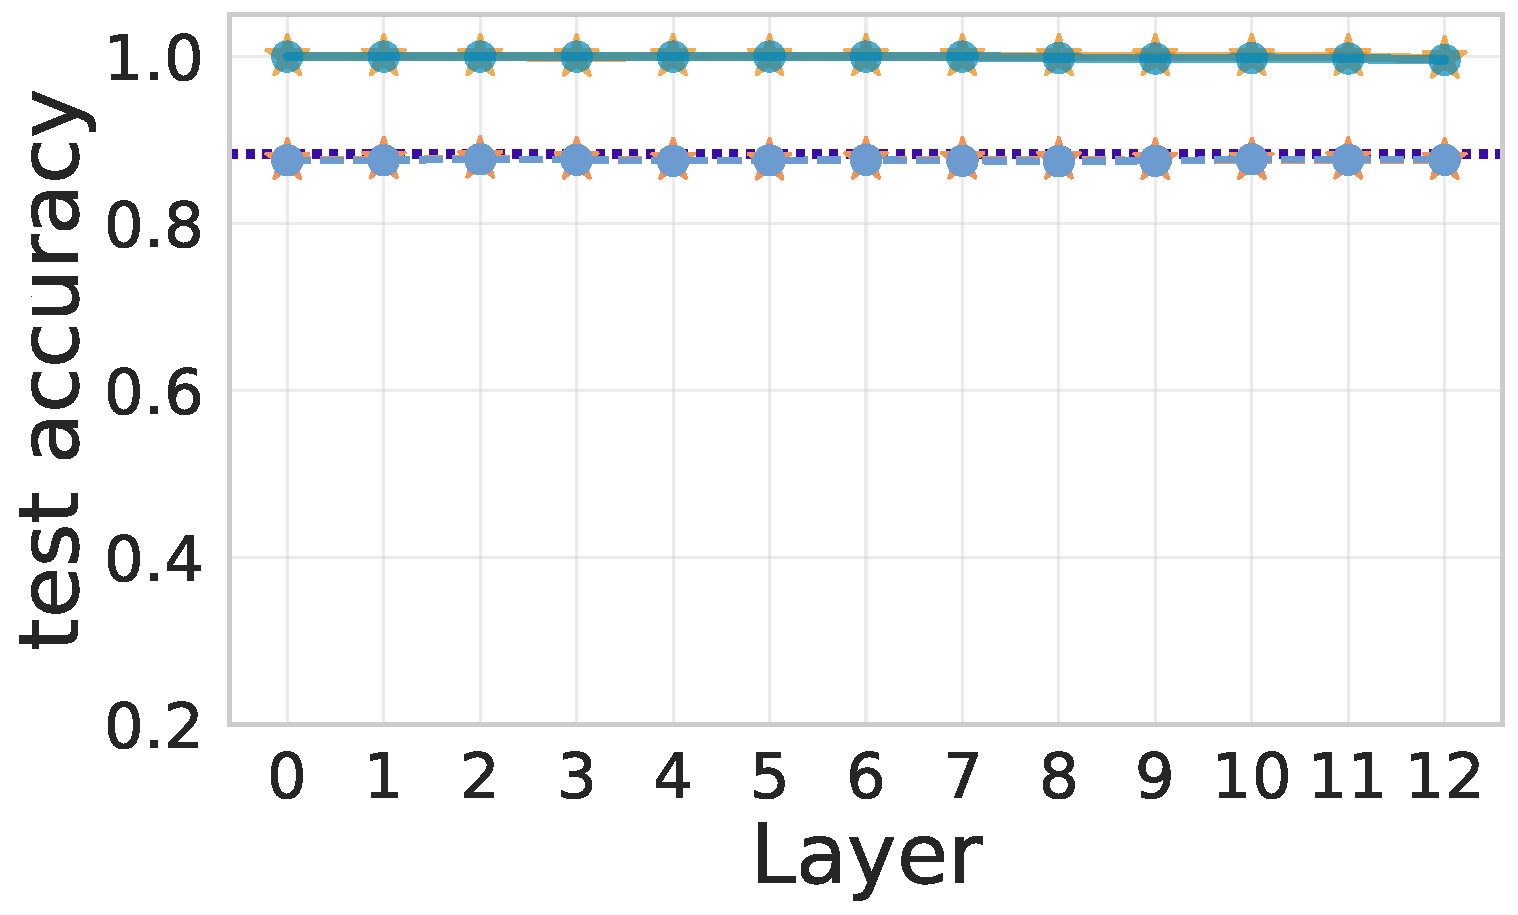
\includegraphics[width=\linewidth]{results_combined/is_aromatic.pdf}
    \subcaption{is aromatic}
    \label{fig:acc-is-aromatic}
\end{subfigure}\hfill
\begin{subfigure}[t]{0.24\textwidth}
    \centering
    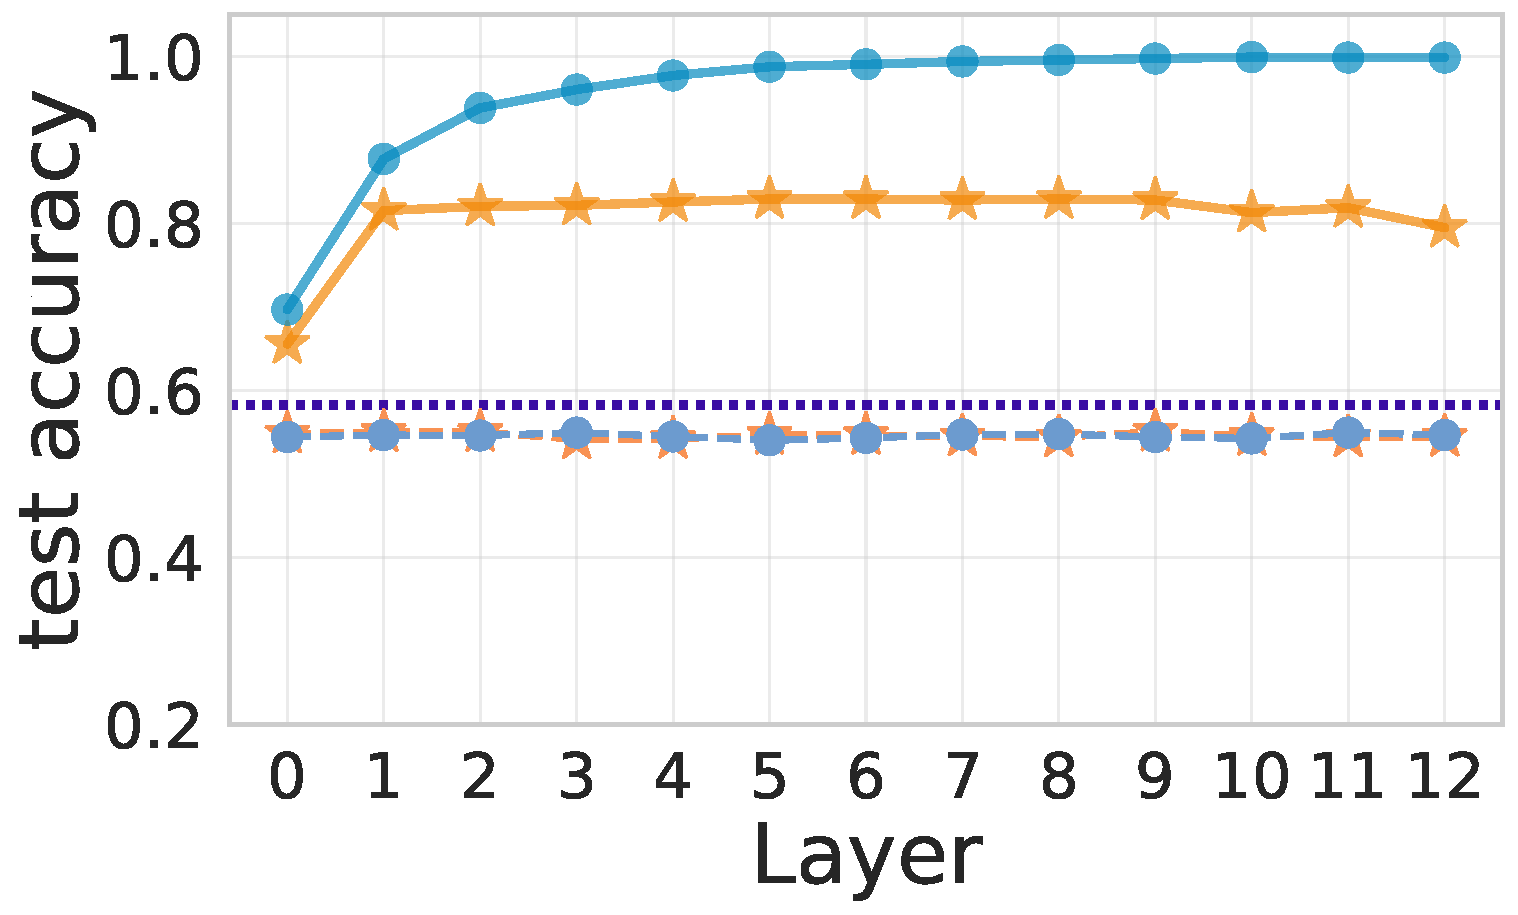
\includegraphics[width=\linewidth]{results_combined/is_in_ring.pdf}
    \subcaption{is in ring}
    \label{fig:acc-is-in-ring}
\end{subfigure}\hfill
\begin{subfigure}[t]{0.24\textwidth}
    \centering
    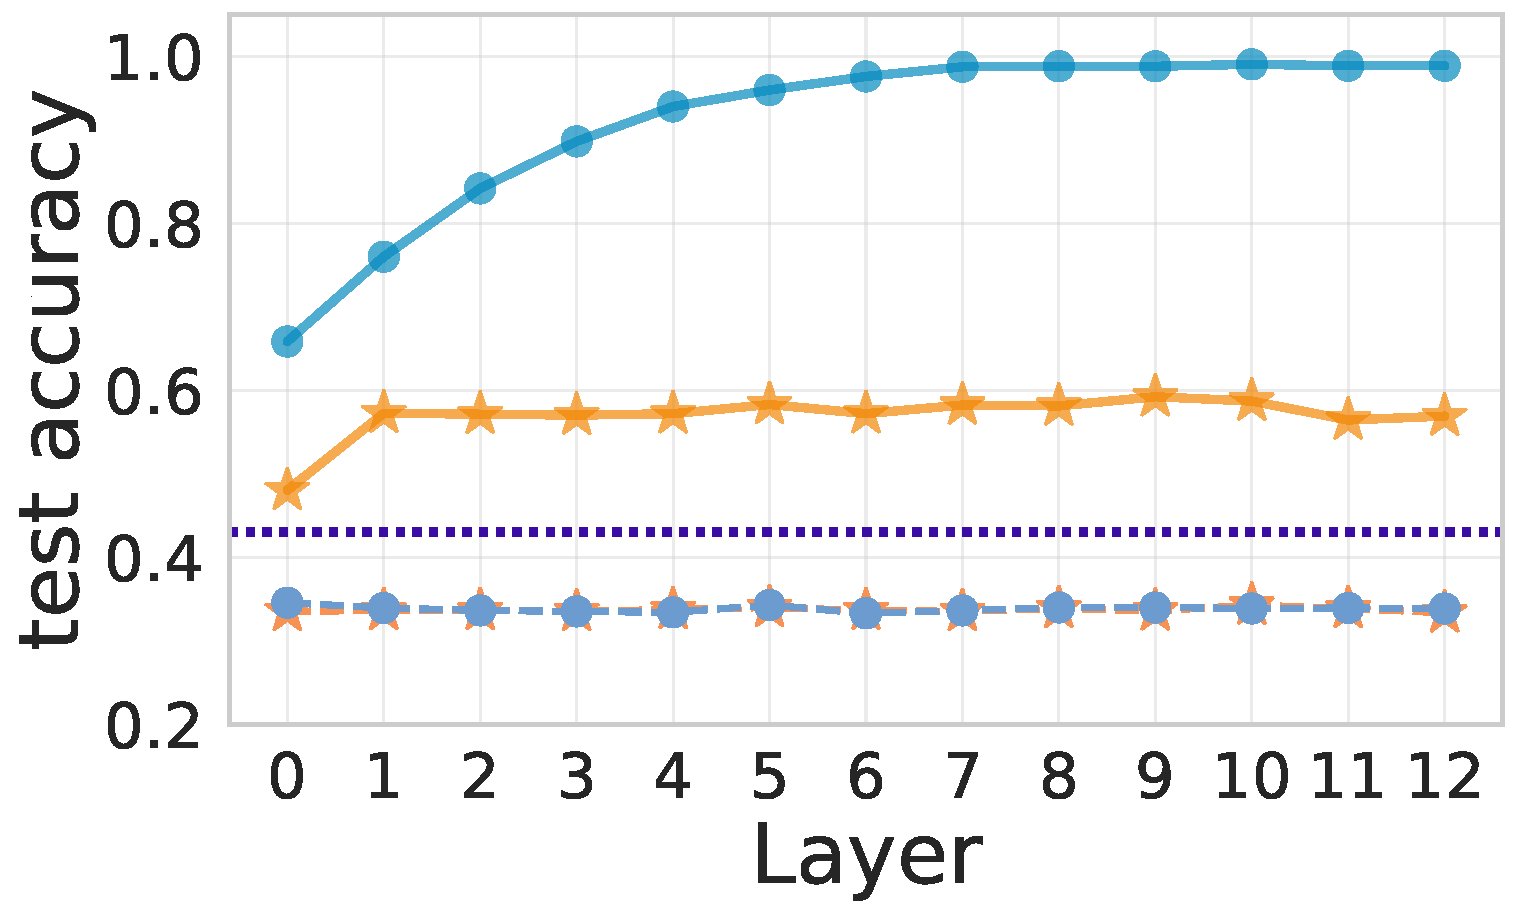
\includegraphics[width=\linewidth]{results_combined/degree.pdf}
    \subcaption{degree}
    \label{fig:acc-degree}
\end{subfigure}\hfill
\begin{subfigure}[t]{0.24\textwidth}
    \centering
    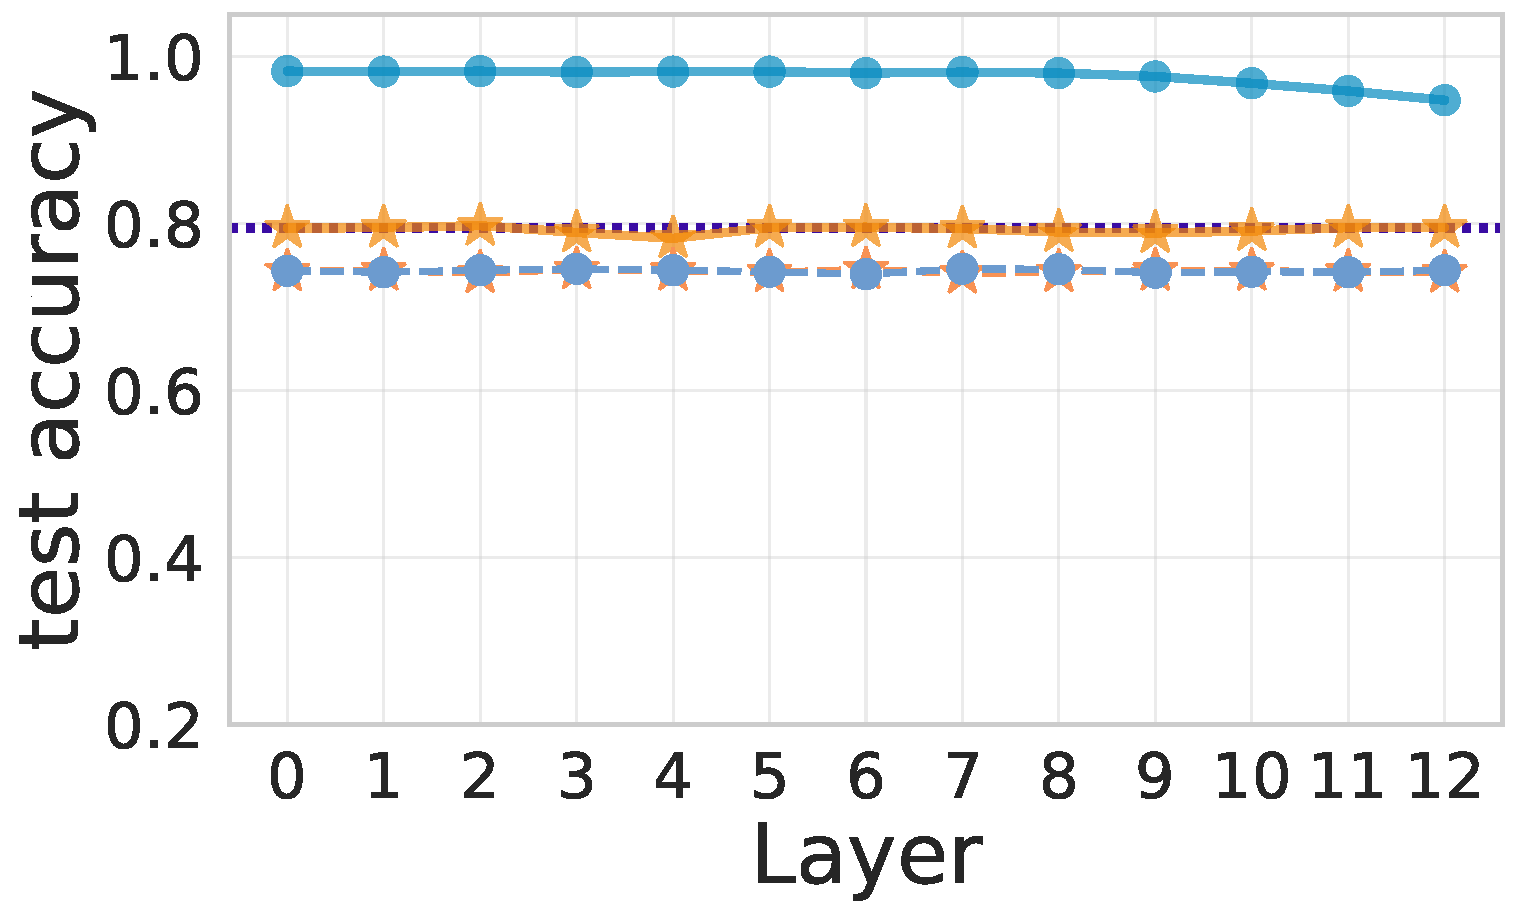
\includegraphics[width=\linewidth]{results_combined/chiral_tag.pdf}
    \subcaption{chiral tag}
    \label{fig:acc-chiral-tag}
\end{subfigure}

\vspace{0.4em}

\begin{subfigure}[t]{0.24\textwidth}
    \centering
    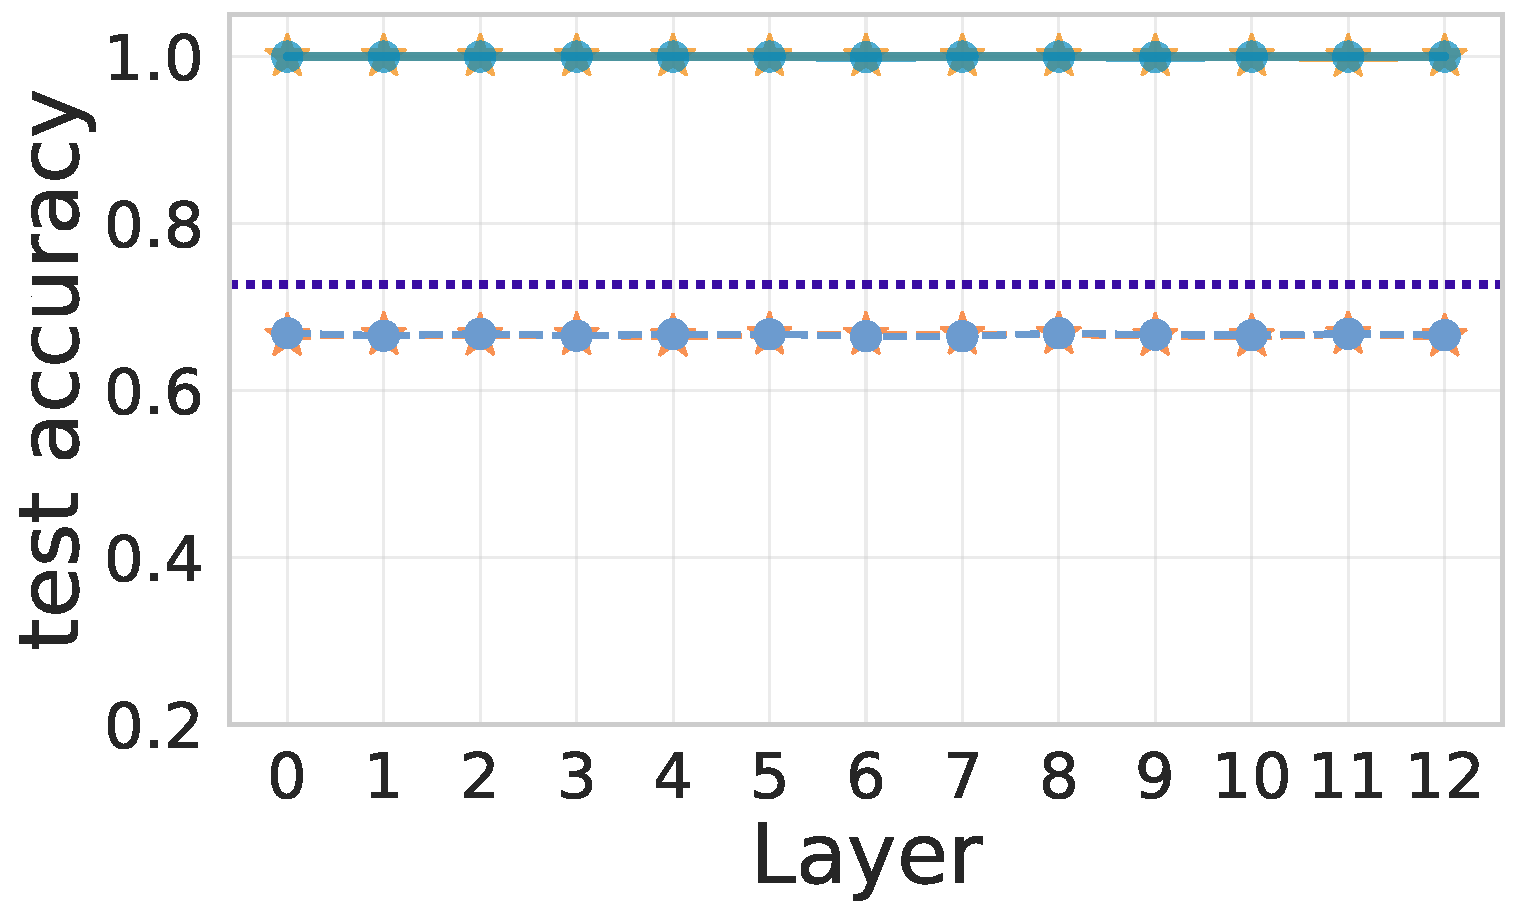
\includegraphics[width=\linewidth]{results_combined/atom_type.pdf}
    \subcaption{atom type}
    \label{fig:acc-atom-type}
\end{subfigure}\hfill
\begin{subfigure}[t]{0.24\textwidth}
    \centering
    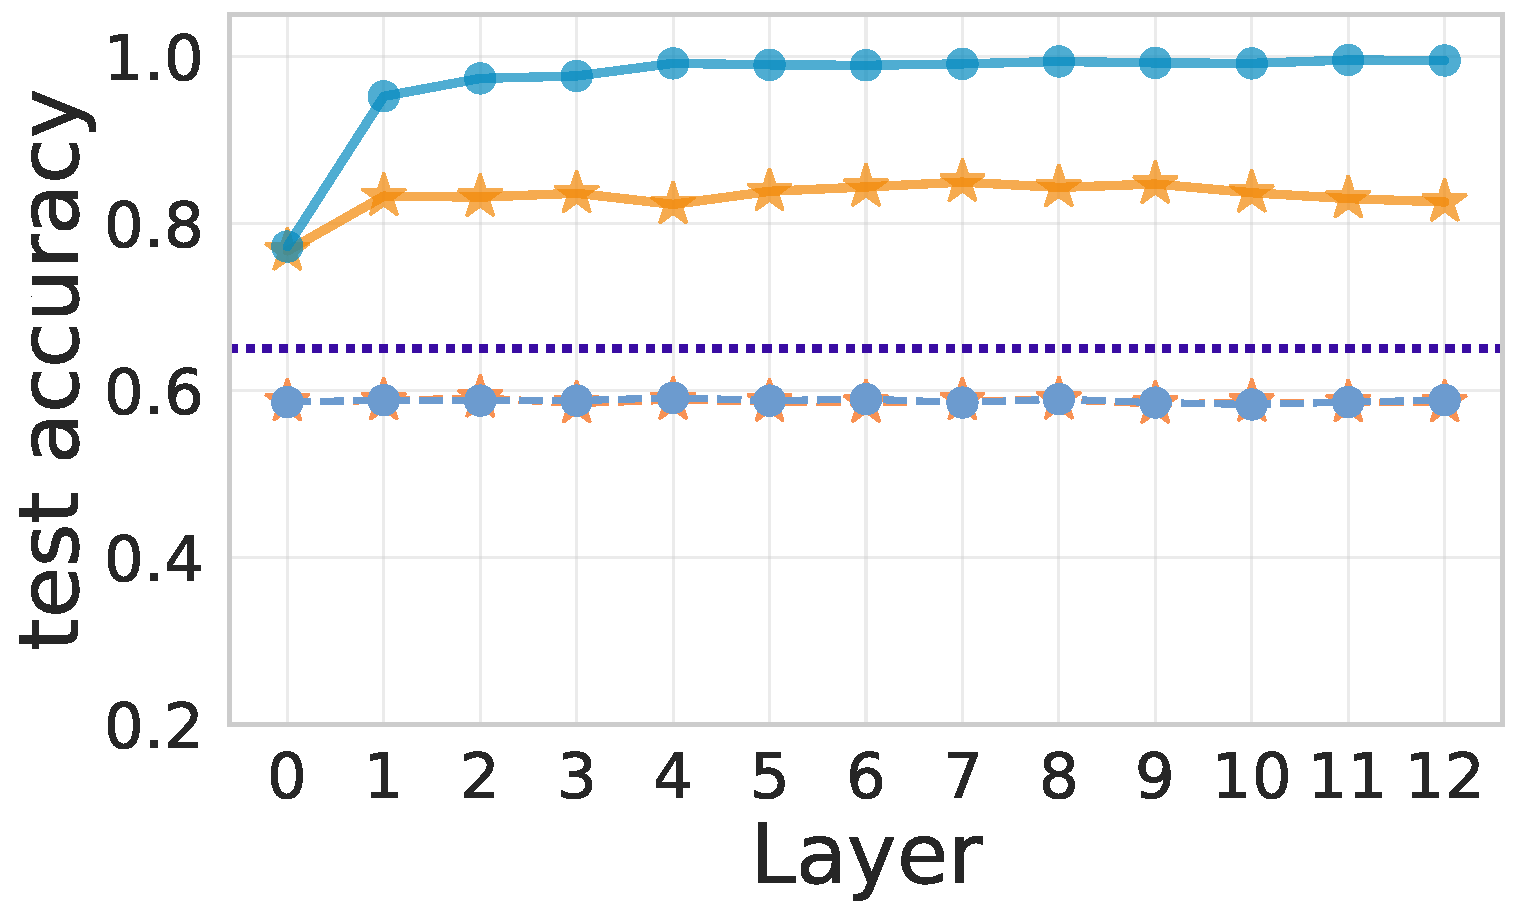
\includegraphics[width=\linewidth]{results_combined/hybridization.pdf}
    \subcaption{hybridization}
    \label{fig:acc-hybridization}
\end{subfigure}\hfill
\begin{subfigure}[t]{0.24\textwidth}
    \centering
    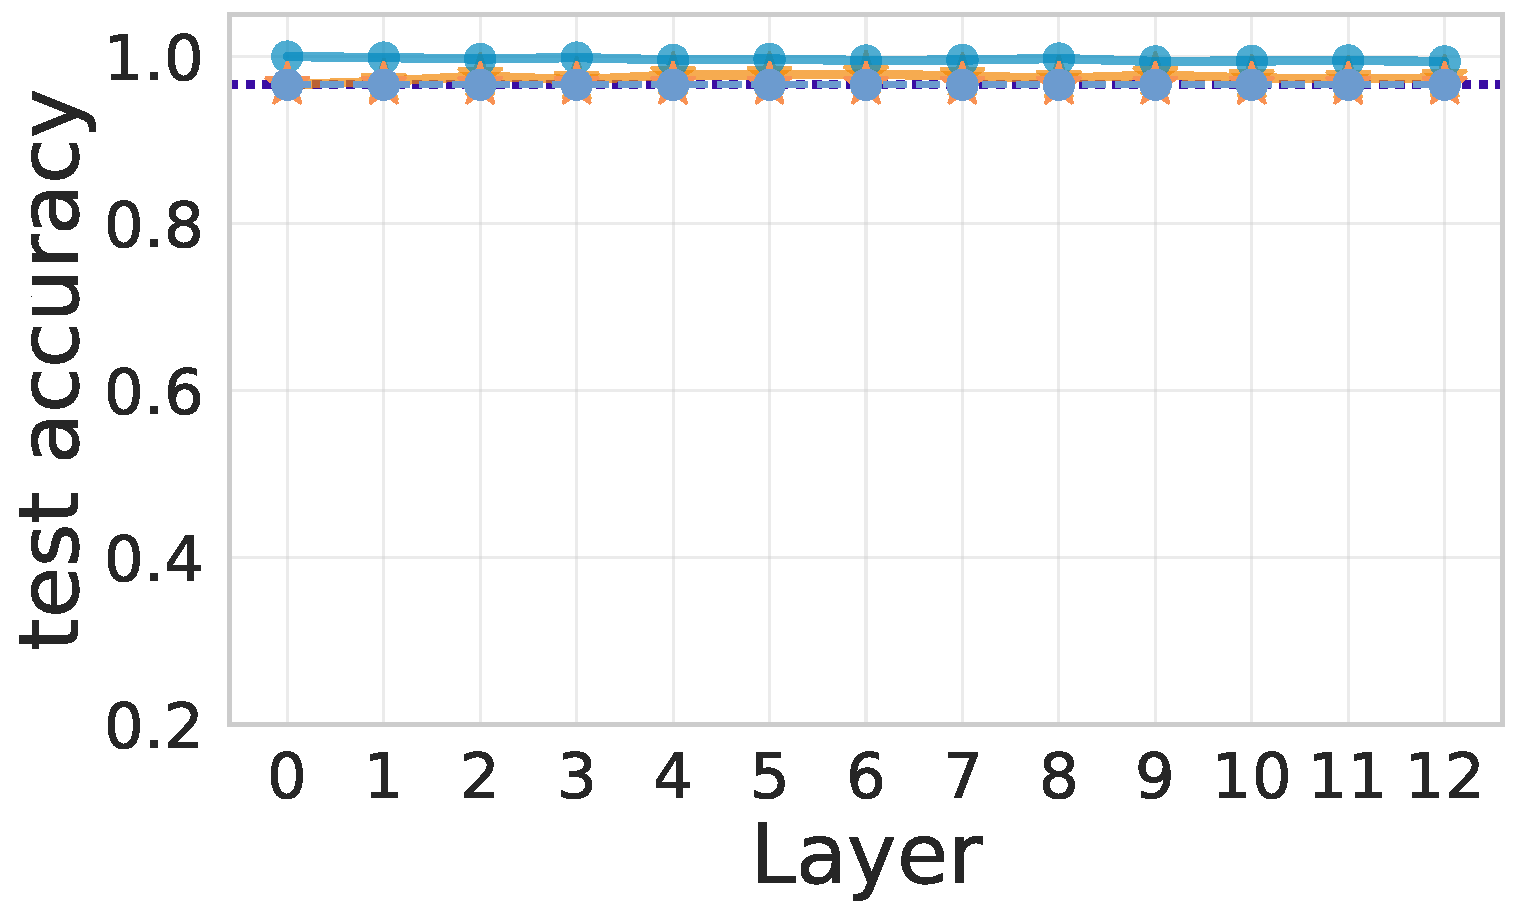
\includegraphics[width=\linewidth]{results_combined/formal_charge.pdf}
    \subcaption{formal charge}
    \label{fig:acc-formal-charge}
\end{subfigure}\hfill
\begin{subfigure}[t]{0.24\textwidth}
    \centering
    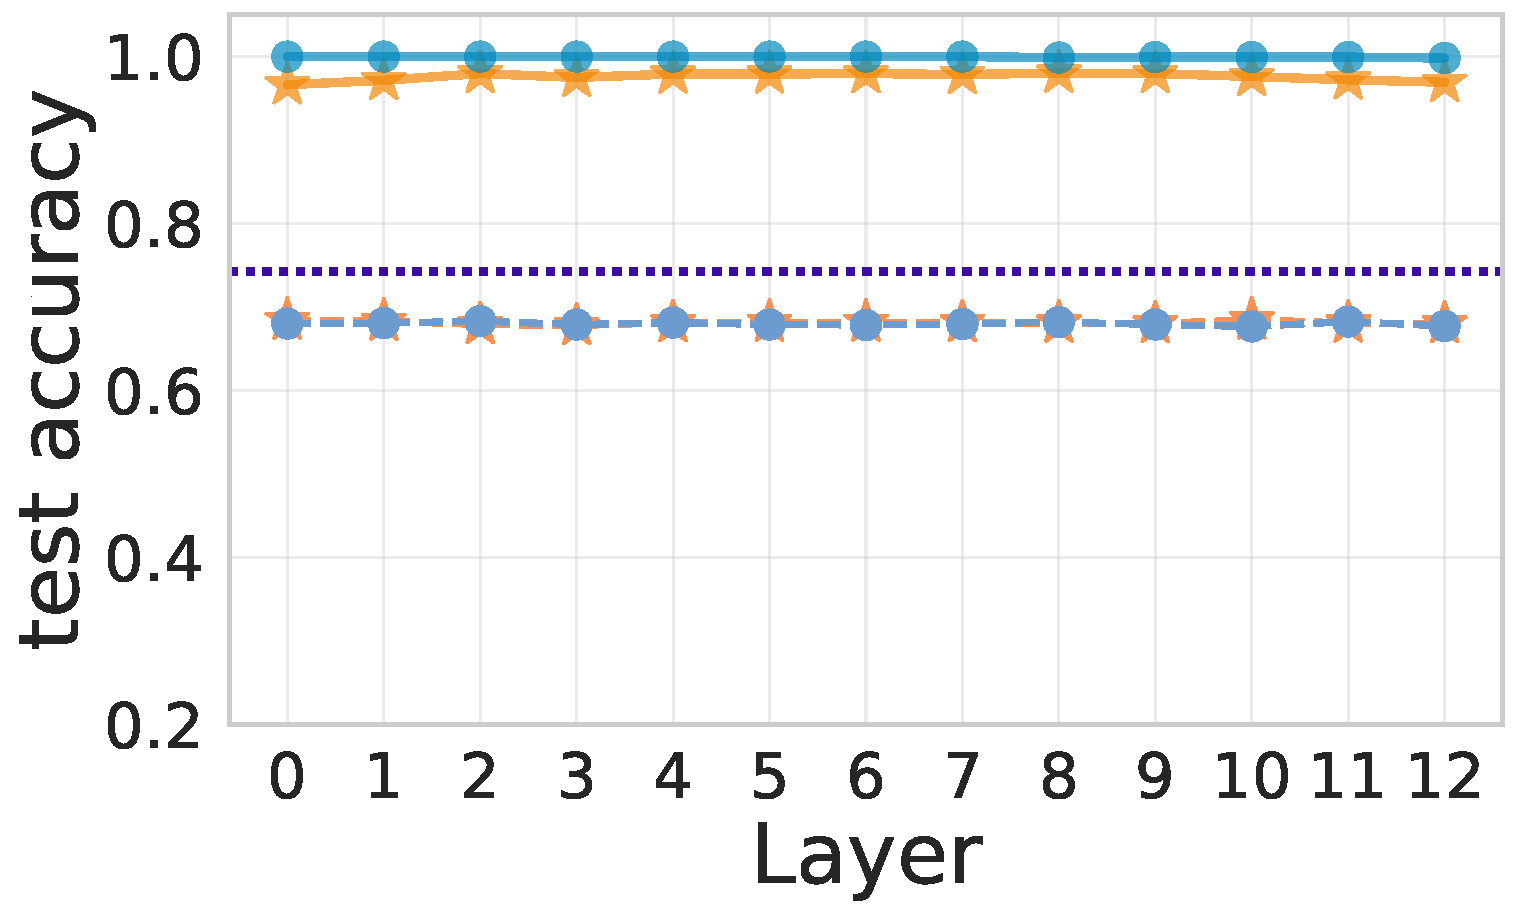
\includegraphics[width=\linewidth]{results_combined/total_valence.pdf}
    \subcaption{total valence}
    \label{fig:acc-total-valence}
\end{subfigure}

\vspace{0.4em}

\centerline{
\includegraphics[width=0.9\textwidth]{results_combined/legend.pdf}}

\caption{Linear-probe test accuracy per layer on eight per-atom QM9 properties. \smi reaches near-perfect accuracy by mid-layers on the contextual properties (ring membership, degree, chiral tag, hybridization, total valence), while \molm plateaus several points below; the surface-form properties (atom type, aromaticity) saturate at the embedding in both models.}
\label{fig:acc}
\end{figure*}


\para{Some properties can be read directly from the SMILES string.}
Aromaticity (Figure~\ref{fig:acc-is-aromatic}) reaches $100\%$ test accuracy at layer~$0$ in both \molm and \smi and remains flat across depth. The SMILES tokenizer encodes aromaticity through letter case (lowercase \texttt{c}, \texttt{n}, \texttt{o}, etc.\ for aromatic atoms), so a single token already carries the label; no encoder computation is needed. Atom type and formal charge sit in the same regime: each element symbol is a distinct token, so probe accuracy is at $100\%$ from the embedding for atom type and at $0.97$--$1.00$ for formal charge (the majority class is already $0.97$). Probe accuracy on these tasks reflects tokenizer design rather than learned representation, and we move them to Appendix~\ref{app:probe-all}.

\para{\smi encodes contextual properties more cleanly than \molm.}
The clearest cross-model gap appears on properties that cannot be read from a single SMILES token: ring membership, degree, and chiral tag (Figure~\ref{fig:acc-is-in-ring}, \ref{fig:acc-degree}, \ref{fig:acc-chiral-tag}). The same \texttt{C} token can belong to a ring or not, can have different degree, and can carry different stereochemistry depending on its surroundings, so a probe that achieves high accuracy on these tasks must read information that the encoder put there from context. \smi reaches near-perfect accuracy by mid-layers on all three (and on hybridization in Appendix~\ref{app:probe-all}), while \molm plateaus around $0.85$, $0.85$, $0.85$, and $0.62$, respectively. The MLP probe (Appendix~\ref{app:mlp}) and the random-features control (Appendix~\ref{app:random}) confirm the gap is not an artifact of probe capacity: the MLP probe improves on the linear probe by at most $0.03$ accuracy across all (task, layer) pairs, and random-features probes collapse to majority-class performance. Given the architectures are nearly identical, the difference plausibly stems from pretraining producing more linearly organized representations of context-dependent structure in \smi.

The probe-only conclusion is, however, partial: it locates information but does not show that the encoder uses it. We resolve this in the next subsection.

\subsection{Causal intervention: what is used}
\label{sec:res-steer}
\begin{figure*}[t]
\centering
\begin{subfigure}[t]{0.24\textwidth}
    \centering
    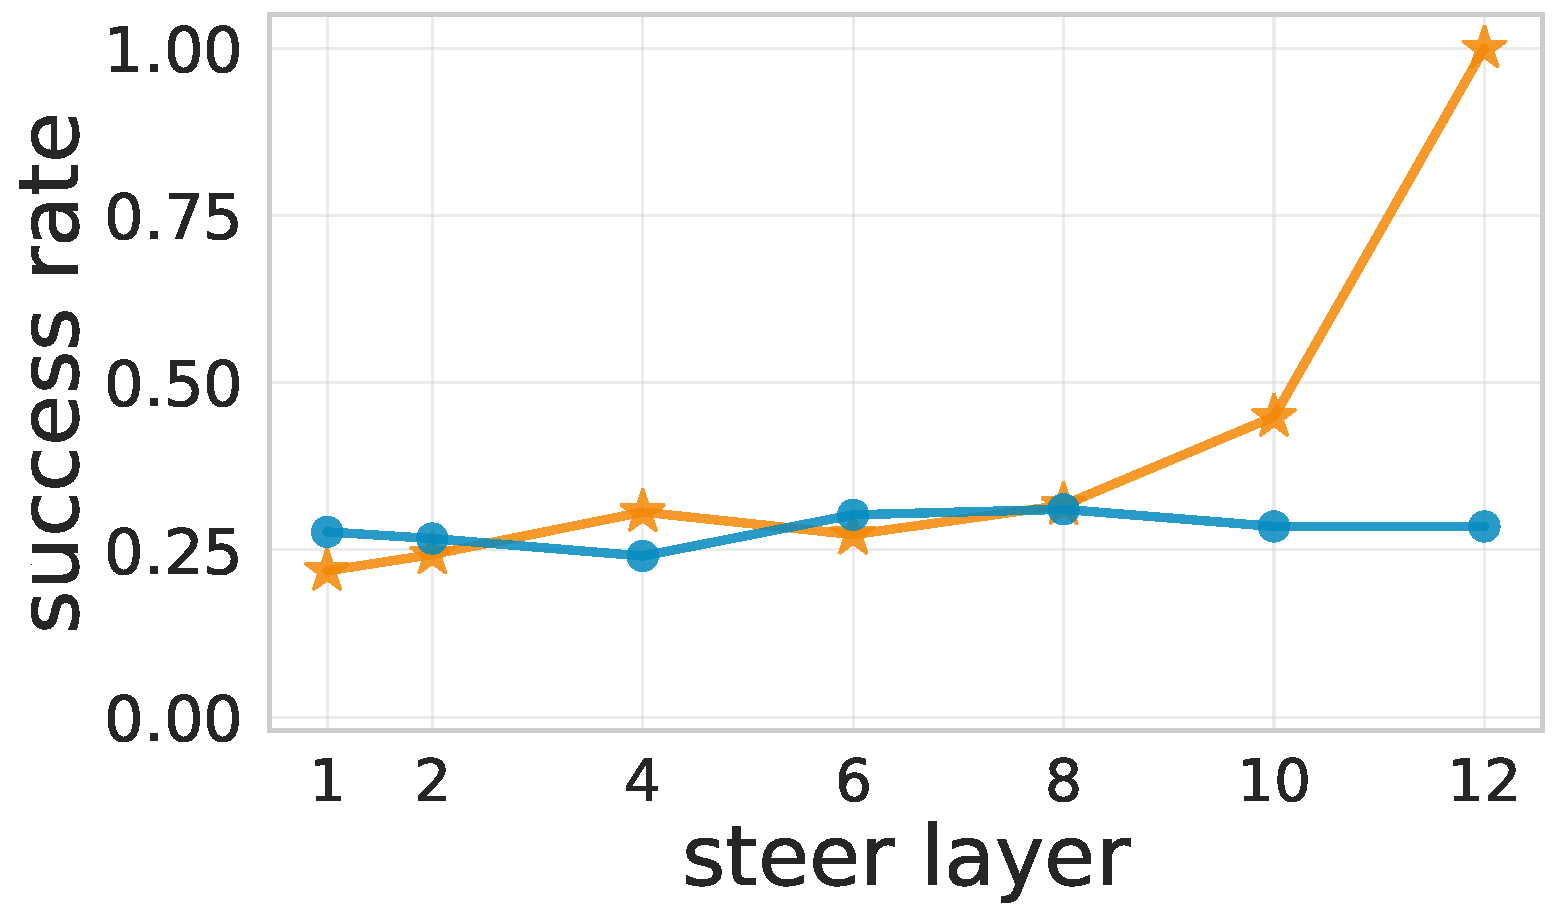
\includegraphics[width=\linewidth]{results_steer_layers/by_layer_atom_type.pdf}
    \subcaption{atom type}
\end{subfigure}\hfill
\begin{subfigure}[t]{0.24\textwidth}
    \centering
    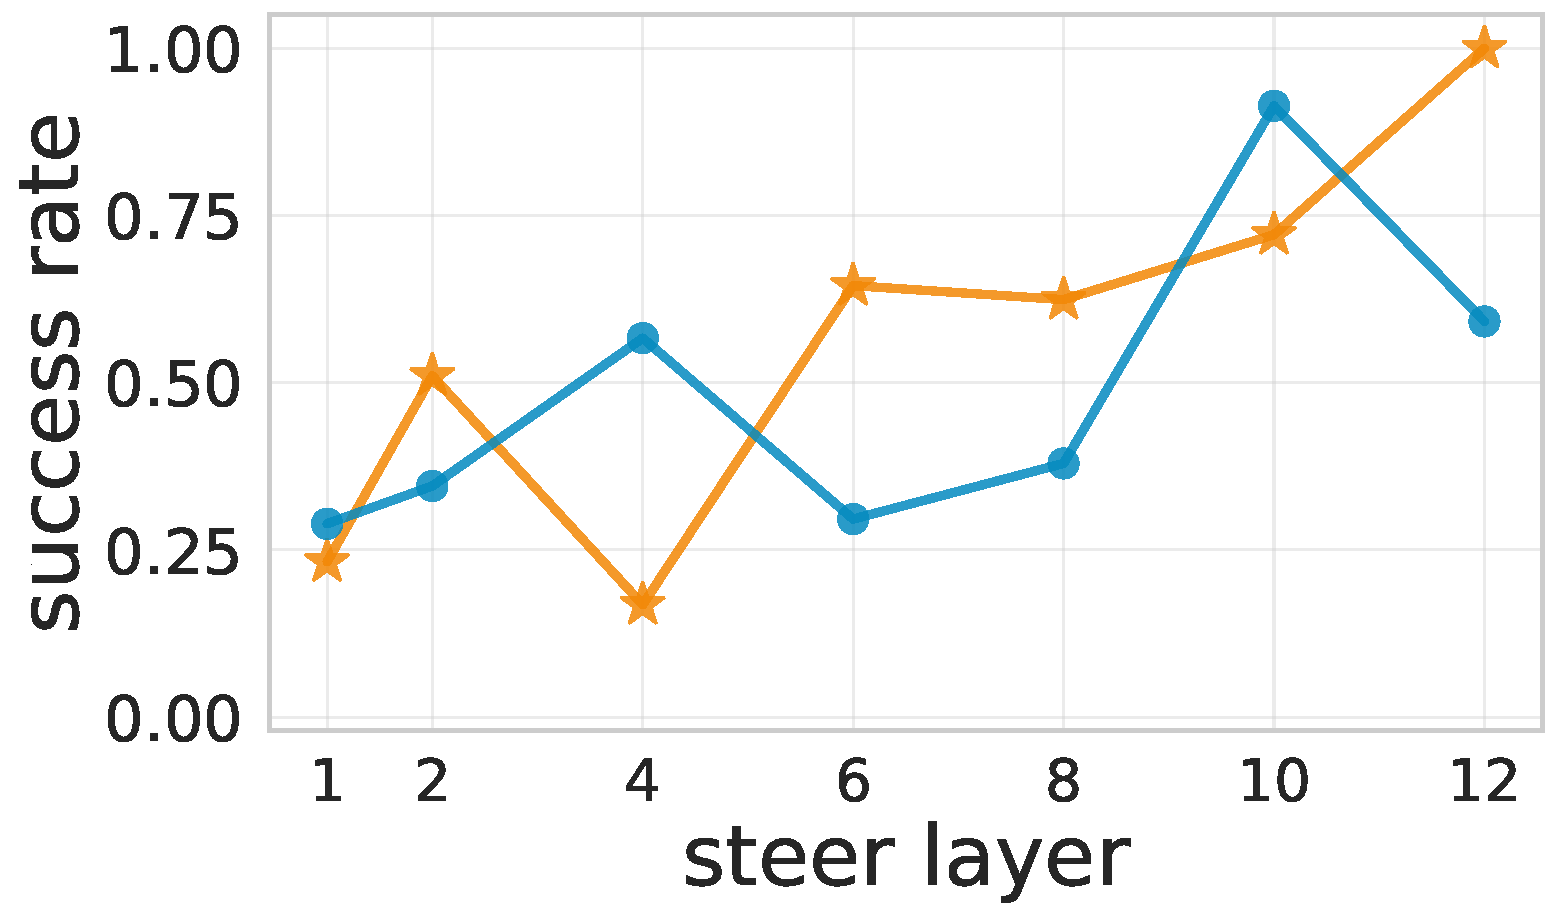
\includegraphics[width=\linewidth]{results_steer_layers/by_layer_hybridization.pdf}
    \subcaption{hybridization}
\end{subfigure}\hfill
\begin{subfigure}[t]{0.24\textwidth}
    \centering
    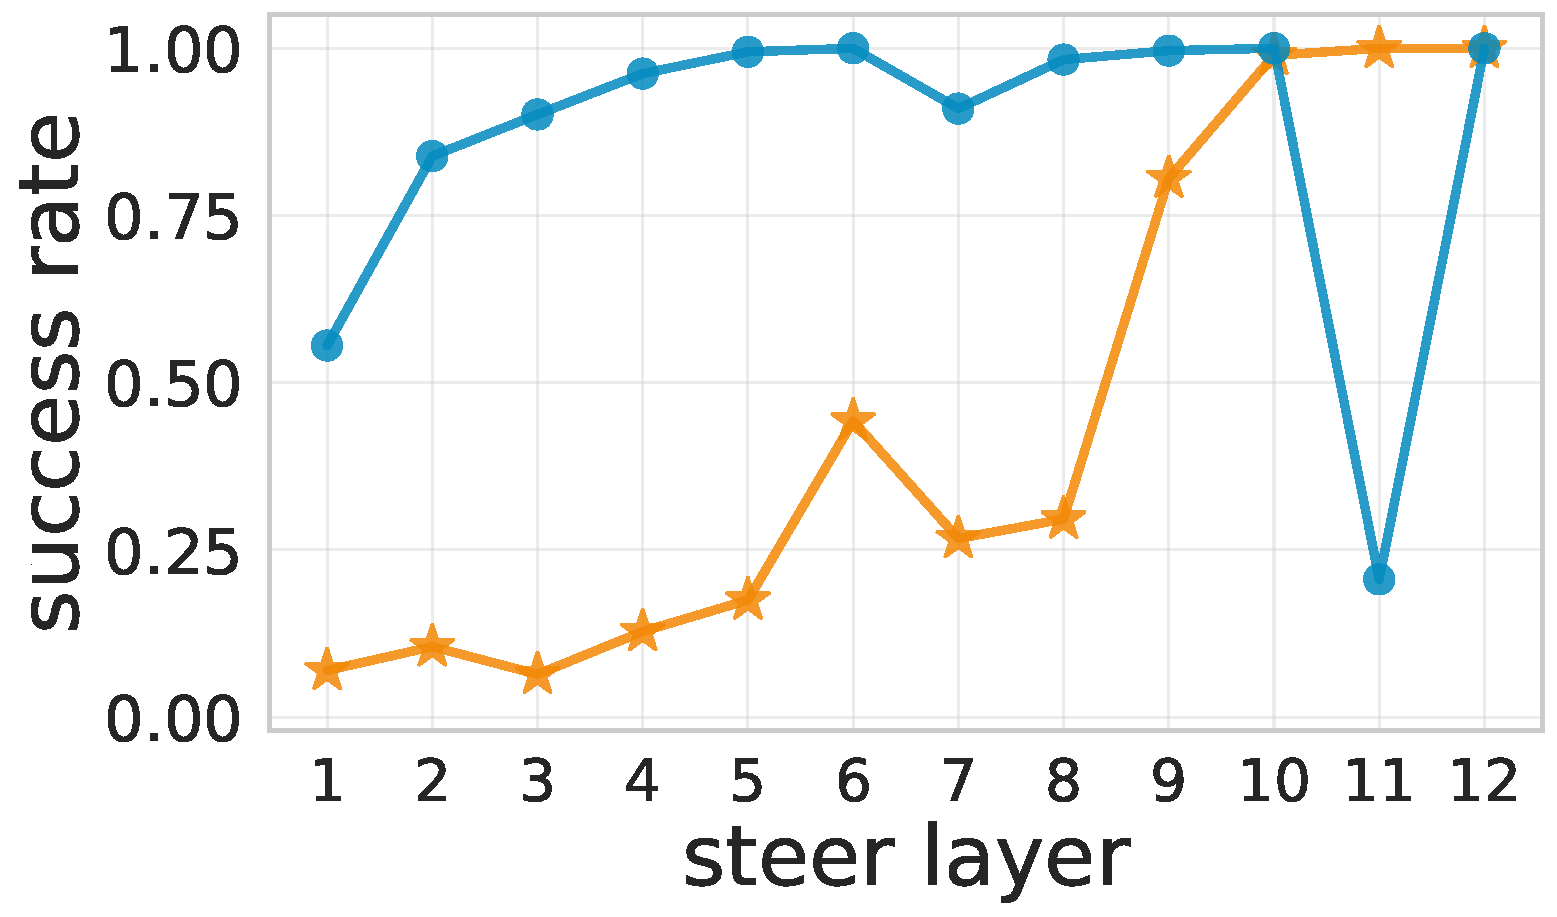
\includegraphics[width=\linewidth]{results_steer_layers/by_layer_chiral_tag.pdf}
    \subcaption{chiral tag}
\end{subfigure}\hfill
\begin{subfigure}[t]{0.24\textwidth}
    \centering
    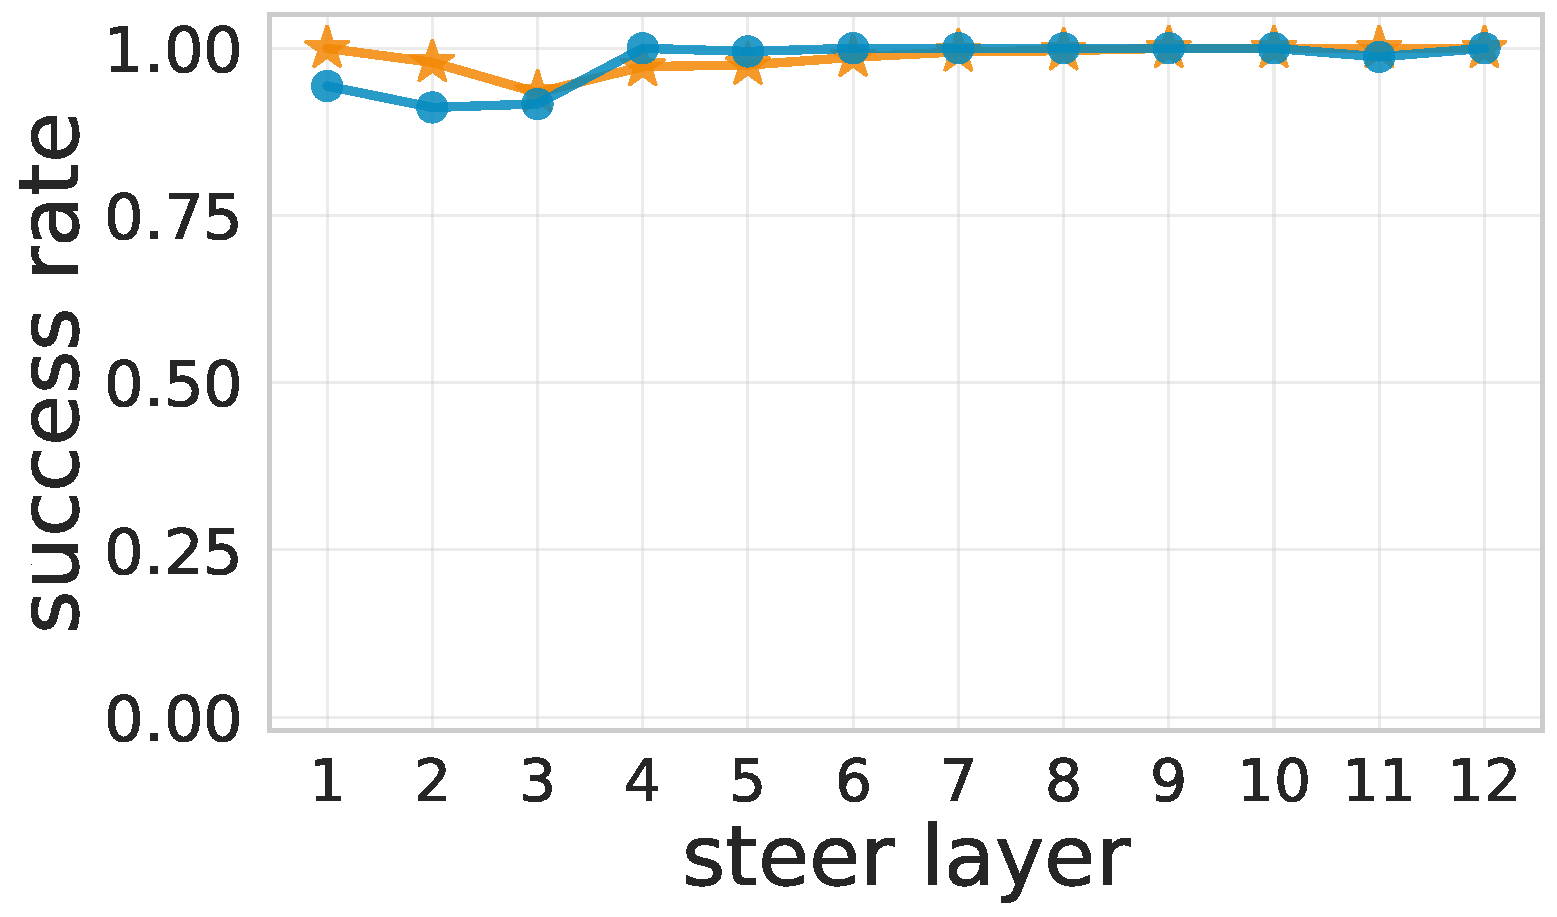
\includegraphics[width=\linewidth]{results_steer_layers/by_layer_is_aromatic.pdf}
    \subcaption{is aromatic}
\end{subfigure}
\vspace{0.6em}

\begin{subfigure}[t]{0.24\textwidth}
    \centering
    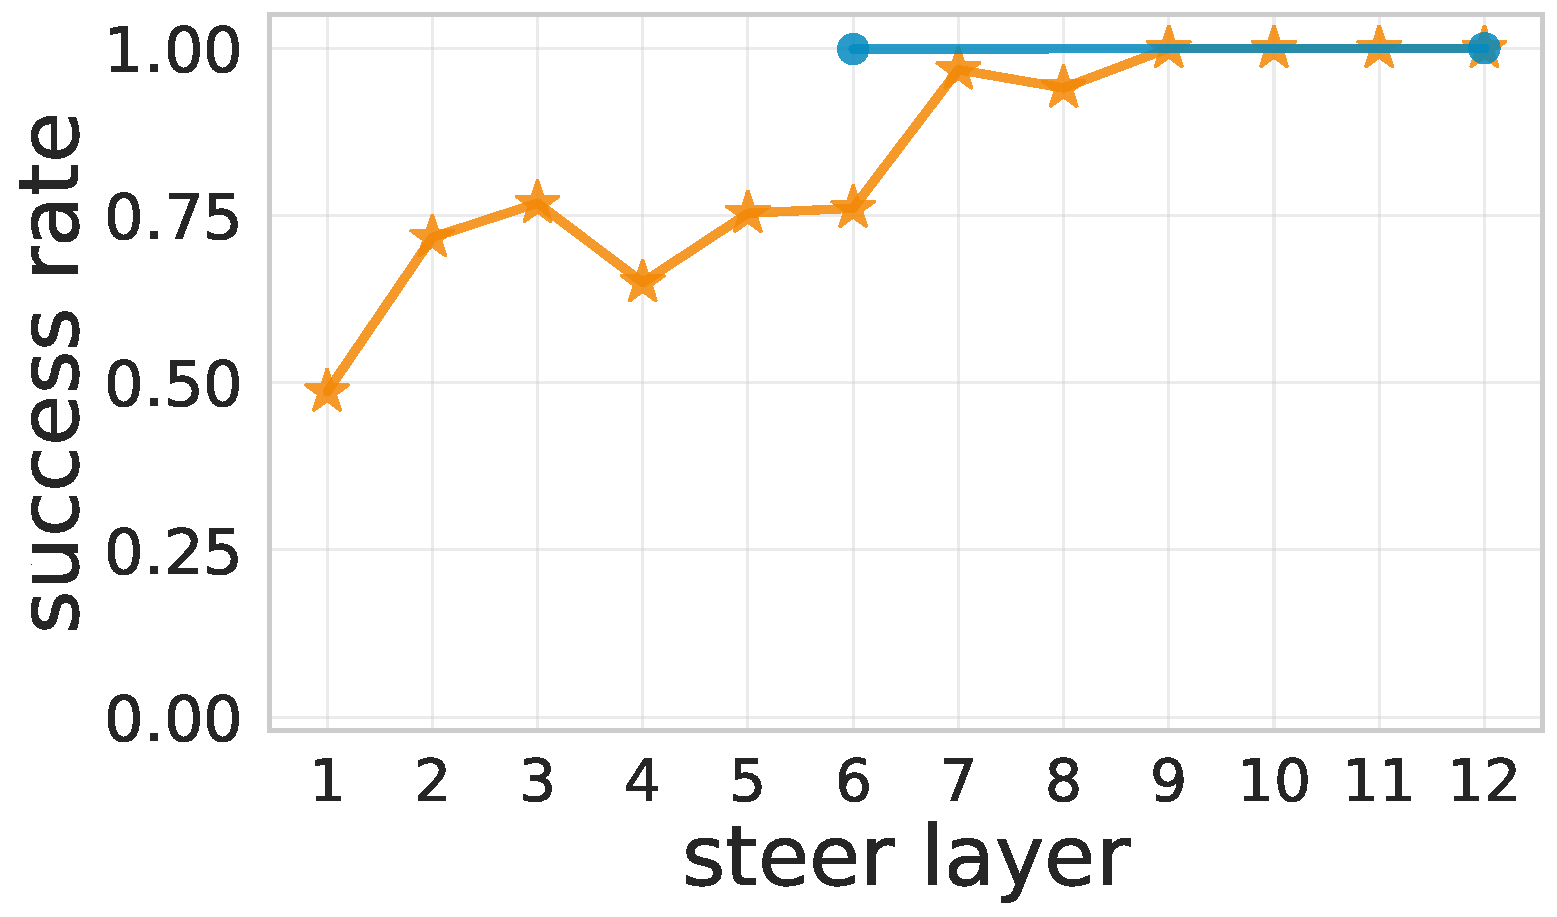
\includegraphics[width=\linewidth]{results_steer_layers/by_layer_is_in_ring.pdf}
    \subcaption{is in ring}
\end{subfigure}\hfill
\begin{subfigure}[t]{0.24\textwidth}
    \centering
    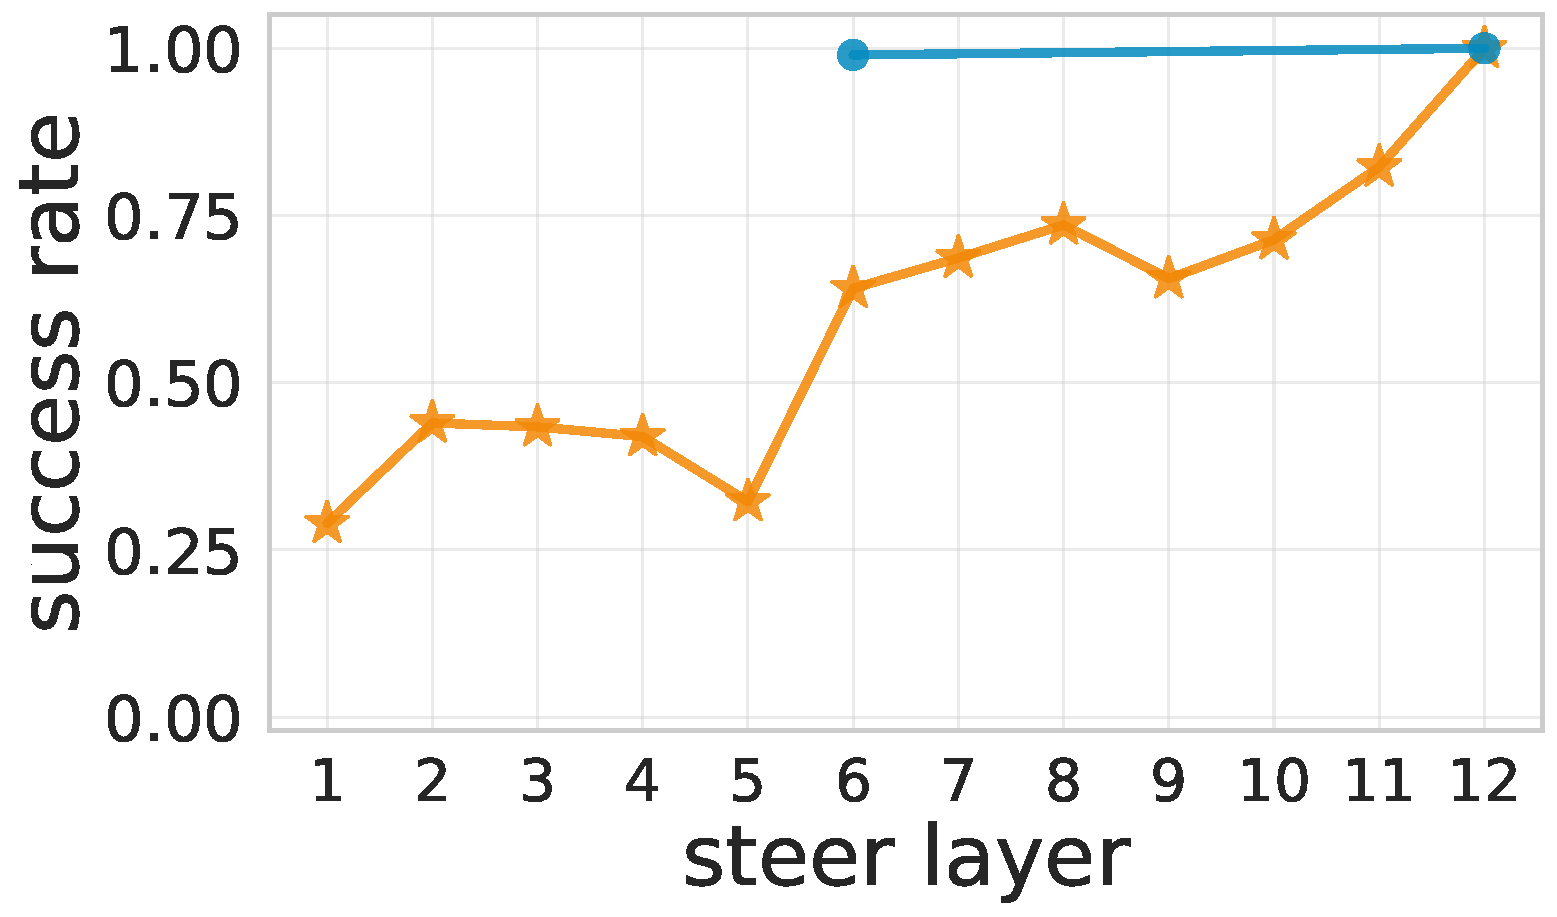
\includegraphics[width=\linewidth]{results_steer_layers/by_layer_degree.pdf}
    \subcaption{degree}
\end{subfigure}\hfill
\begin{subfigure}[t]{0.24\textwidth}
    \centering
    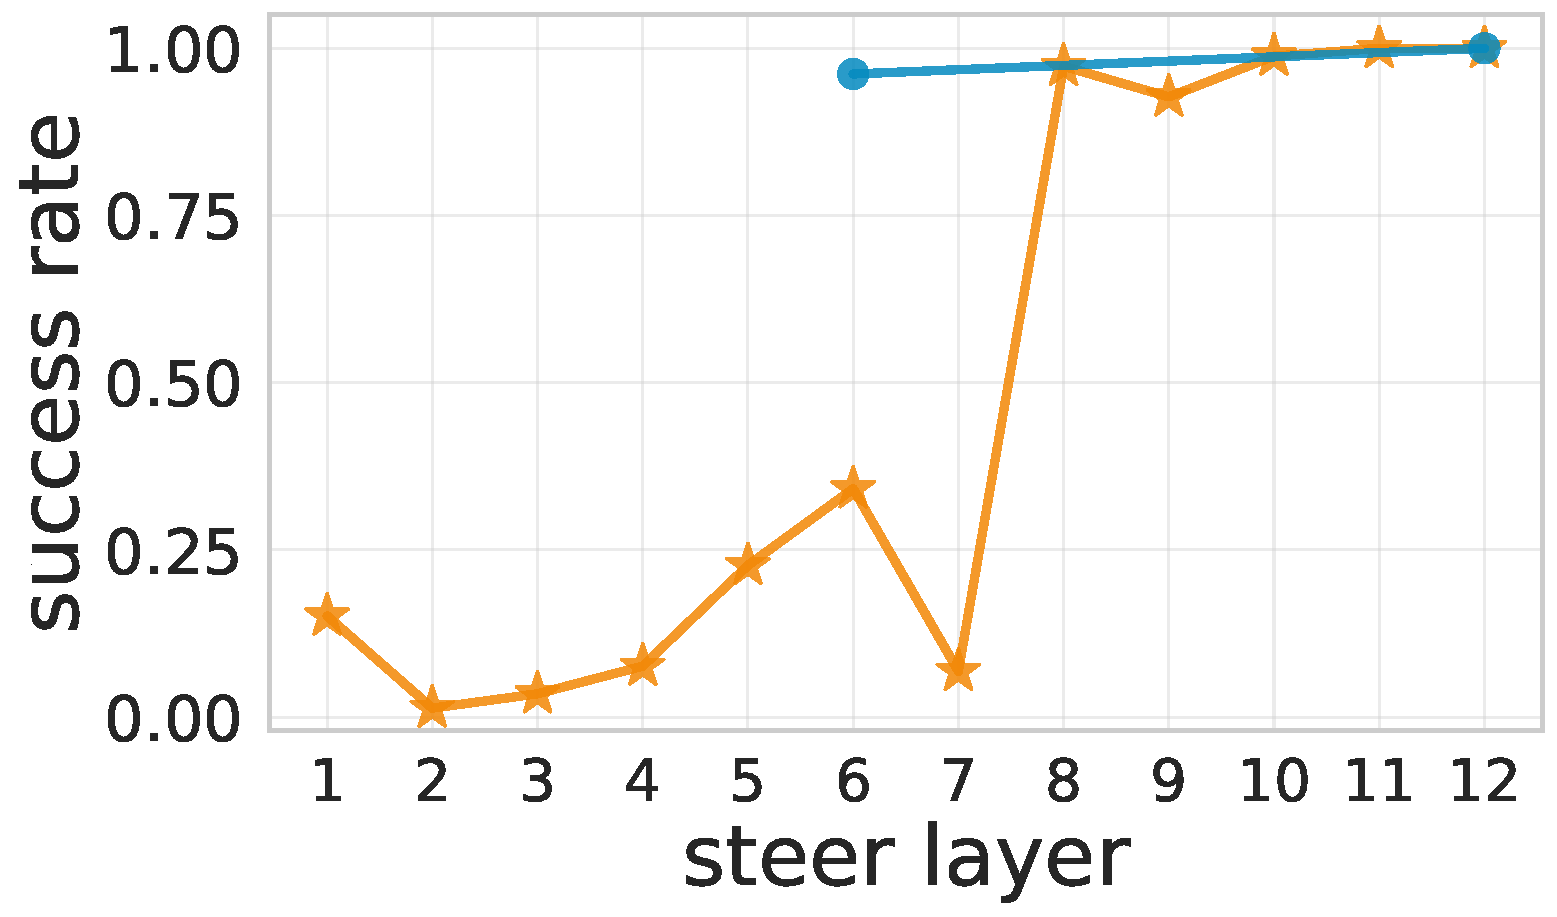
\includegraphics[width=\linewidth]{results_steer_layers/by_layer_formal_charge.pdf}
    \subcaption{formal charge}
\end{subfigure}\hfill
\begin{subfigure}[t]{0.24\textwidth}
    \centering
    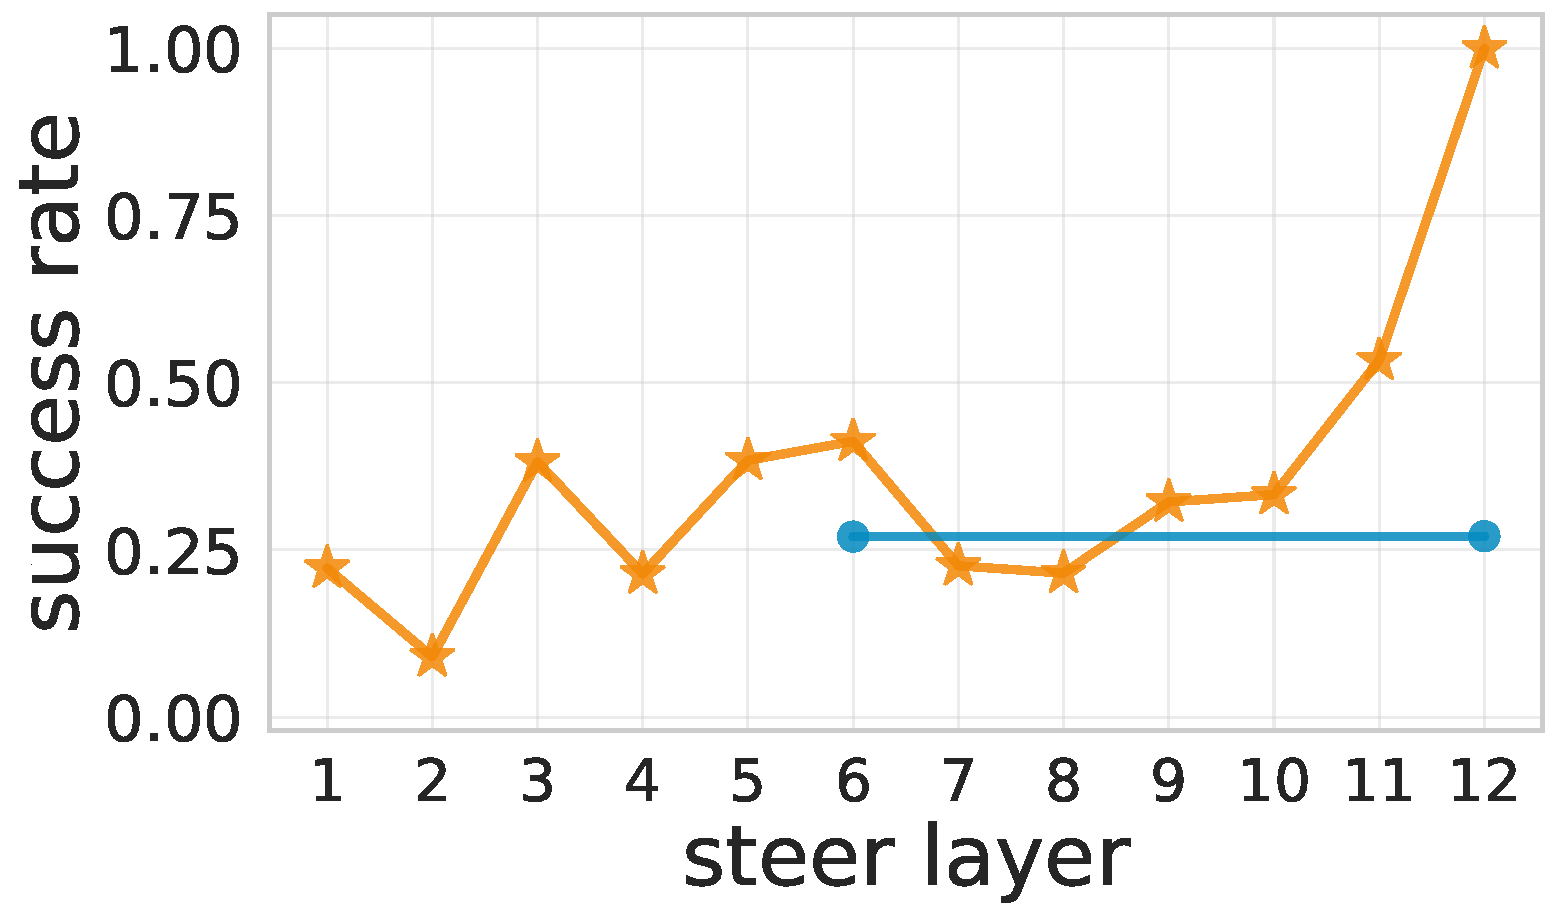
\includegraphics[width=\linewidth]{results_steer_layers/by_layer_total_valence.pdf}
    \subcaption{total valence}
\end{subfigure}

\vspace{0.4em}

\centerline{
\includegraphics[width=0.5\textwidth]{results_steer_layers/by_layer_legend.pdf}}

\caption{\textbf{Intervention success rate as a function of the steer layer.} For each (task, model, layer~$\ell$) we intervene at $\ell$ along the layer-$\ell$ probe direction and read the layer-$12$ probe; the curve plots the best success rate over $\alpha$ on $200$ held-out QM9 molecules. \smi's curve is flat near~$1$ on all binary contextual tasks (ring membership, aromaticity), meaning the probed direction is a usable channel at \emph{every} depth. \molm's ring-membership curve climbs from $\sim 0.5$ at layer~$1$ to $1.00$ by layer~$9$, indicating the information is causally used only at the deepest layers despite being partially decodable throughout. Multi-class tasks (atom type, hybridization, total valence) include a probe-prototype geometry confound on the cycle target and are interpreted with that caveat in the text.}
\label{fig:steer-layer}
\end{figure*}


For each (task, source class $c$, target class $c'$, steer layer $\ell$) we add $\alpha \cdot (\mathbf{W}_{c'}-\mathbf{W}_{c})/\boldsymbol{\sigma}$ at every atom-token position whose baseline prediction is $c$, run the rest of the encoder, and read the layer-$12$ probe; \emph{intervention success rate} is the fraction of those positions whose post-intervention layer-$12$ prediction equals $c'$. For binary tasks $c'$ is the only other class; for multi-class tasks we use a cycle target $c' = (c + 1) \bmod C$. Setup, hook implementation, and the per-source moved-off-source diagnostic are in Appendix~\ref{app:steering}. Single-layer interventions at $\ell{=}6$ already reproduce the probing-level ranking on contextual binary tasks (ring membership: $76\%$ on \molm, $100\%$ on \smi; Table~\ref{tab:steering-success} in Appendix~\ref{app:steering}).

\para{Sweeping the steer layer localizes \emph{where} information is causally used.}
A single-layer intervention can only confirm or deny encoder use at that depth; it cannot say where else the property is causally available. We therefore sweep $\ell \in \{1, \ldots, 12\}$ and report, for each (task, model, $\ell$), the intervention success rate at the best-performing $\alpha$ on the held-out molecules (Figure~\ref{fig:steer-layer}).

\emph{Aromaticity} (Figure~\ref{fig:steer-is-aromatic}) gives the trivial baseline. Probe accuracy is $1.0$ from the embedding and intervention success is $\approx 1.0$ at every depth in both models. The probe direction is a usable channel everywhere because the property essentially \emph{is} the embedding.

\emph{Ring membership} (Figure~\ref{fig:steer-is-in-ring}), \emph{degree} (Figure~\ref{fig:steer-degree}), and \emph{chiral tag} (Figure~\ref{fig:steer-chiral-tag}) all show the same pretraining-difference shape. \smi's success rate climbs rapidly through the early layers and saturates at $1.0$ by mid-depth, in lockstep with the probe reaching near-perfect accuracy: the probed direction is treated as a usable channel by the encoder from mid-layers onward. \molm's success rate, by contrast, climbs gradually and only reaches $1.0$ at the top of the encoder, even though its mid-layer probe accuracy (around $0.85$) is roughly constant across that range. The probe finds a partial linear correlate at every depth in \molm, but only the deepest layers give the encoder a direction that subsequent computation routes through.

\subsection{Discussion: encoded versus used}
\label{sec:res-disc}

The two measurements jointly carve up our observations. When probe accuracy is high \emph{and} intervention success is high---aromaticity at every depth in both models, ring membership / degree / chiral tag at and beyond mid-layers in \smi---the property is both encoded and causally used: it is what the rest of the encoder reads. When neither is high, the property is simply not in the representation; we do not see this case in our eight tasks. The interpretively interesting case is the asymmetry: a probe that decodes the property well at a given depth, but an intervention along the same direction that does not control the layer-$12$ readout. The layer sweep is what makes this case interpretable.

\para{Hypothesis: the information is used at a different depth.}
Under this reading the probe at the intervention layer is reading a passive correlate; the encoder's computational channel for the property lives at another depth, typically deeper. The diagnostic is the layer sweep: the depth at which intervention success becomes high is the depth at which the encoder routes through the probed direction. \molm on degree (Figure~\ref{fig:steer-degree}) is the cleanest instance. Probe accuracy is roughly constant ($\approx 0.85$) across mid-layers but intervention success climbs from $0.29$ at layer~$1$ to $1.00$ at layer~$12$: the information is partially encoded throughout but causally used only at the top of the encoder. Ring membership, formal charge, and chiral tag on \molm follow the same shape (Appendix~\ref{app:steer-all}). This is the form of pretraining gap that probing alone obscures: \molm and \smi have qualitatively similar mid-layer probe accuracies on these tasks within an order of magnitude, but only \smi's representations are organized as a usable channel from mid-depth onward.

\para{Synthesis: \smi's pretraining gap is both representational and functional.}
Combining probing and intervention sharpens the qualitative claim made by prior work~\cite{soares2024smi, sharma2025foundation} that \smi's stronger downstream performance reflects better representations. Probing shows \smi encodes contextual properties as cleaner linear directions than \molm. Intervention shows those same directions are routed through every subsequent encoder block in \smi, whereas \molm's are routed only at the deepest layers. The advantage is therefore not located at any single depth or in either measurement alone: it is the joint property of being both \emph{cleanly organized} and \emph{causally used} throughout the encoder, which is what makes the representations more directly available to downstream heads.

\section{Concluding Discussion}
\label{sec:res-disc}

\xiaoyan{Discuss more on the linear probing results and the mismatch between causality test and the probe.}
\anita{Implications paragraph add later}

Taken together, the attention and probing results suggest that chemical information is not represented uniformly across mechanisms or layers in these models. Attention exhibits only weak and highly selective alignment with molecular geometry, indicating that spatial structure is not encoded through a small set of geometry-tracking heads. In contrast, probing and causal intervention reveal that chemically meaningful properties are strongly represented within the residual stream, but become computationally usable at substantially different depths across models. More broadly, our results move beyond asking whether chemical information is present, toward understanding how chemically relevant structure is internally organized and used during computation.

\para{The primary difference between \molm and \smi lies in when chemical information becomes functionally usable.}
Our results suggest that \smi makes contextual chemical information functionally usable substantially earlier in the encoder, whereas \molm often does so only near the top layers. This distinction may matter most for downstream tasks requiring multi-step integration of chemical information. Properties relevant to ADMET prediction, reactivity, and molecular binding often depend on combining multiple local and non-local chemical cues rather than detecting a single motif. When a representation becomes usable early, subsequent layers can build on it as an intermediate computational feature for forming more global or task-specific representations. By contrast, representations that become usable only near the top of the encoder may still support final prediction, but have less opportunity to influence preceding computation.

This distinction may be particularly important in practical transfer settings, where molecular encoders are commonly used through fixed embeddings, shallow predictors, parameter-efficient adaptation, partial freezing, or intermediate-layer readouts rather than fully end-to-end optimization~\cite{honda2019smiles,rollins2024molprop,cai2026chemfm,harod2025effichem,pinto2025unlocking}. Under these constraints, downstream performance may depend less on what information is eventually present in the model and more on which chemical features are already accessible, and at what depth. Layerwise functional accessibility may therefore be an important predictor of downstream robustness, transferability, and data efficiency.

% \para{These findings also suggest design principles for better chemistry foundation models.}
% First, tokenizer-aware evaluation is essential. Some properties appear at layer~0 because they are already specified by token identity, and these cases should not be treated as evidence of learned chemical abstraction. More informative benchmarks are contextual properties that require integration beyond the local token. Second, pretraining should be evaluated not only by final task accuracy, but also by whether it produces simple and persistent internal features that remain usable across depth. This perspective favors objectives and architectures that encourage early integration of relational structure rather than deferring chemically meaningful computation to the final layers. Third, the weak attention-distance correlations highlight a limitation of standard SMILES-only pretraining: strong predictive performance does not necessarily imply a spatially grounded internal representation. If spatial reasoning is the target capability, stronger geometric inductive bias or multimodal 3D supervision may be required.

\para{Future Directions.}
One natural next step is to study the internal geometry of chemical representations more directly. While linear probing identifies which properties are recoverable, it does not characterize how different chemical features are arranged relative to one another within representation space, whether they occupy shared or independent subspaces, or how these structures evolve across layers. Future work could examine feature overlap, representation superposition, and layerwise organization using methods such as sparse autoencoders, subspace analysis, or representation similarity techniques.

A second direction is to trace how chemical information flows through the network during computation. Our causal interventions show when a representation becomes functionally usable, but do not yet identify which downstream components consume that information or how multiple chemical features are composed into higher-level reasoning. Studying attention circuits, residual-stream interactions, and feature propagation across layers may help reveal how models combine local chemical descriptors into more global molecular representations.

Finally, an important open question is how different pretraining choices shape the resulting internal representations. Although \molm{} and \smi{} achieve similar downstream performance, they differ substantially in when and how chemical information becomes usable. Extending this analysis to additional architectures, objectives, and training datasets may help identify which design choices lead to more structured, transferable, or computationally efficient chemical representations.


% TODO

%%%%%%%%%%%%%%%%%%%%%%%%%%%%%%%%%%%%%%%%%%%%%%%%%%%%%%%%%%%%
\section*{Impact Statement}
%%%%%%%%%%%%%%%%%%%%%%%%%%%%%%%%%%%%%%%%%%%%%%%%%%%%%%%%%%%%

\bibliography{main}
\bibliographystyle{icml2026}

\newpage
\appendix
\onecolumn
\section{Models and Atomic Properties}
\label{appendix:architecture}

\para{\molm{}.}
\molm{}~\citep{ross2022largescalechemicallanguagerepresentations} is an encoder-only transformer that applies rotary linear attention to SMILES token sequences and produces both token-level hidden states and a pooled molecular representation. The public release we study has a 12-layer encoder with hidden size 768 and 12 attention heads, and a vocabulary of $2{,}362$ tokens. The encoder is pretrained on roughly 1.1 billion molecules from PubChem~\citep{kim2023pubchem} and ZINC~\citep{sterling2015zinc} under a masked language modeling objective, with no explicit supervision on geometry or molecular properties. Each token is embedded in a $768$-dimensional space, and sequences are capped at $202$ tokens, which accommodates over $99.4\%$ of molecules in the training corpus.
\molm{} replaces standard softmax attention with a positive-feature-map approximation~\citep{choromanski2021rethinking}, combined with rotary position encodings $R_m$ applied to queries and keys at each position $m$. The resulting attention at position $m$ is
\begin{equation}
\text{Attention}_m(Q, K, V) = \frac{\sum_{n=1}^{N} \langle \varphi(R_m q_m),\, \varphi(R_n k_n) \rangle\, v_n}{\sum_{n=1}^{N} \langle \varphi(R_m q_m),\, \varphi(R_n k_n) \rangle},
\end{equation}
where $\varphi$ is a random feature map that enables linear-time attention and avoids the quadratic cost of standard softmax attention.

\para{\smi{}.}
\smi{}~\citep{soares2024smi} uses the same general encoder backbone (12 layers, $768$-dimensional hidden states, 12 attention heads, rotary linear attention) but adds an encoder--decoder bottleneck trained jointly with token-level prediction and sequence reconstruction. The encoder maps token embeddings $\mathbf{x}$ into a compressed latent representation $\mathbf{z}$ via
\begin{equation}
\mathbf{z} = \mathrm{LayerNorm}\!\left(\mathrm{GELU}\!\left(\mathbf{x} W_1 + b_1\right)\right) W_2,
\end{equation}
and reconstructs the token sequence from $\mathbf{z}$ through a symmetric immersion followed by a language decoder layer. The encoder contains $47$M parameters and the decoder $242$M parameters, totalling $289$M parameters. This bottleneck imposes an additional constraint on the latent space: it must retain enough information to support both downstream prediction and recovery of the input SMILES, which makes \smi{} a useful comparison point for studying whether different pretraining designs lead to different internal organization of chemical information.

\para{Why this comparison is informative.}
The two models are similar enough at the architectural level that layerwise comparisons are meaningful: same depth, same hidden size, same attention mechanism, and SMILES-only inputs without explicit geometric supervision. They differ in how molecular information is pooled and constrained during pretraining, which lets us attribute representational differences to pretraining choices rather than architectural ones.

\subsection{Atomic Properties Derived from RDKit}
\label{appendix:properties}

Each atom is annotated with eight RDKit-derived properties, falling into three categories of how readable they are from the SMILES string itself.

\para{Surface-form (directly recoverable from SMILES tokenization).}
\textbf{Atom type} is the chemical element identity of the atom. Element symbols are explicitly encoded in the SMILES string and assigned distinct token ids by the tokenizer, so atom type is directly readable.
\textbf{Aromaticity} indicates whether an atom belongs to an aromatic system; aromatic atoms are written with lowercase letters in SMILES notation, so aromaticity is also surface-form.

\para{Partially signaled by SMILES.}
\textbf{Formal charge} is the net charge assigned to an atom relative to its neutral state. It is sometimes indicated by bracket notation, but consistent labels require RDKit standardization across representations.
\textbf{Chiral tag} encodes the stereochemical configuration at a chiral center. SMILES partially signals chirality with \texttt{@} and \texttt{@@}, but canonical assignment requires stereochemical perception by RDKit.

\para{Contextual (require cheminformatics computation).}
\textbf{Hybridization} describes the orbital hybridization state of an atom; aromatic atoms implicitly carry sp$^2$ character via lowercase notation, but hybridization for non-aromatic atoms requires full valence resolution.
\textbf{Degree} is the number of directly bonded heavy-atom neighbors of each atom; while bond connectivity is encoded in SMILES, degree must be computed by parsing the molecular graph since implicit hydrogens complicate direct reading.
\textbf{Total valence} counts all bonds formed by an atom, including bonds to implicit hydrogens, which SMILES typically suppresses.
\textbf{Ring membership} indicates whether an atom belongs to one or more rings; SMILES encodes ring closures through numbered bond descriptors, but assigning ring membership to each atom (especially in fused or bridged polycyclic systems) requires explicit ring perception.

The five contextual properties (and partially-signaled formal charge and chiral tag) cannot be determined from raw SMILES alone, and therefore serve as the most informative targets for evaluating how much structural information a model has learned beyond its tokenization. We additionally consider one geometric property, \textbf{interatomic distance}, in our attention analysis (Appendix~\ref{app:attention-overall}); this property is not encoded in the SMILES string at all and must be estimated from a generated 3D conformer.

\section{Attention--Distance Details}
\label{app:attention-appendix}

We test whether attention preferentially connects atoms that are spatially close in 3D. For each layer--head pair $(l,h)$, we compute the Spearman correlation between attention weights and inverse interatomic distance across all unique heavy-atom pairs $i<j$, then average these correlations across molecules. We randomly sample 1000 SMILES strings from the QM9 training split, excluding molecules with fewer than three heavy atoms, and apply the same procedure to both models.

\para{Attention extraction.}
Both \molm and \smi use the FAVOR$+$ linear-attention approximation~\citep{choromanski2021rethinking}, which does not explicitly materialize the full attention matrix. We therefore capture the query and key tensors $\mathbf{q}_i^{(l,h)}$ and $\mathbf{k}_j^{(l,h)}$ at every layer and head, reconstruct the effective attention weights post hoc as
$
A_{ij}^{(l,h)} \propto \langle \varphi(\mathbf{q}_i^{(l,h)}), \varphi(\mathbf{k}_j^{(l,h)}) \rangle,
$
and apply row normalization. We restrict attention to atom-token rows and columns, discarding non-atomic tokens.

\para{Conformer generation.}
Because SMILES strings encode molecular connectivity but not 3D geometry, we generate a single low-energy conformer for each molecule using RDKit ETKDGv3 followed by MMFF94 optimization, assigning each heavy atom coordinates $\mathbf{r}_i = (x_i,y_i,z_i)$.

\para{Distance correlation.}
From the optimized conformer, we compute the pairwise Euclidean distance matrix
$
D_{ij} = \|\mathbf{r}_i - \mathbf{r}_j\|_2,
$
form the inverse-distance matrix $D^{-1}$, and compute the Spearman correlation between $\{A_{ij}^{(l,h)}\}$ and $\{1/D_{ij}\}$ over all unique heavy-atom pairs $i<j$. We additionally stratify correlations by short-range ($\leq 2$\,\AA), medium-range ($2$--$4$\,\AA), and long-range ($>4$\,\AA) interactions to localize where geometric signal is concentrated.

\para{Summary.}
Both models exhibit only weak overall alignment between attention and 3D geometry, with the strongest correlations concentrated in short- and medium-range atom pairs.

\section{Probing and Causal Intervention Details}
\label{app:training}
\label{app:mlp}
\label{app:random}
\label{app:steering}
\label{app:probe-all}
\label{app:steer-all}

\subsection{Probe training and data}

\para{Optimization.} Each linear probe is a single fully-connected layer $\mathbf{W}\in\mathbb{R}^{C_\tau \times d}$, $\mathbf{b}\in\mathbb{R}^{C_\tau}$ trained from random initialization for every (task, layer) pair under cross-entropy loss. We use AdamW with learning rate $10^{-3}$, weight decay $10^{-2}$, batch size $256$, $50$ epochs, and gradient norm clipping at $5.0$. The MLP probe and the random-features probe (described below) use the same optimizer, schedule, and standardization as the linear probe.

\para{Data and split.} We sample $1000$ SMILES uniformly at random from the QM9 training split with seed $42$. After RDKit parsing and atom-token alignment, approximately $980$ molecules and $\sim 8.6$k atom-token positions remain. We use a molecule-level $80/20$ split so that no atom from a held-out molecule appears in training, yielding $\sim 6.9$k training and $\sim 1.7$k test atom-token positions. Class sets are fit on training labels only; held-out atoms whose label does not appear in training count as misclassifications and are excluded from macro-F1.

\para{Per-atom hidden-state extraction.} For each SMILES we run a forward pass with \texttt{output\_hidden\_states=True}, parse the molecule with RDKit, and align tokenizer-level atom tokens with their RDKit atom indices via a deterministic walk through the regex tokenization. Each atom-token's element symbol is verified against the corresponding RDKit atom; mismatched molecules are dropped. The per-atom vector $\mathbf{h}^{(i)}_{\tau, l} \in \mathbb{R}^{d}$ at layer $l$ is the $i$-th atom-token row of the layer-$l$ hidden-states tensor.

\para{Standardization.} For each (task, layer), per-feature mean $\boldsymbol{\mu}_{\tau, l}$ and standard deviation $\boldsymbol{\sigma}_{\tau, l}$ are computed on training atoms only and applied as $\tilde{\mathbf{h}} = (\mathbf{h} - \boldsymbol{\mu}_{\tau, l}) / (\boldsymbol{\sigma}_{\tau, l} + 10^{-8})$ to both train and test. The $10^{-8}$ term avoids division by zero on near-constant features.

\para{Reproducibility shims.} The public \molm{} release predates \texttt{transformers}~$\geq 5$, so we add three monkey-patches at load time: a stub for the removed \texttt{transformers.onnx} subpackage, a stub for \texttt{find\_pruneable\_heads\_and\_indices}, and a re-injection of \texttt{PreTrainedModel.get\_head\_mask}. We also force a recomputation of the rotary embedding's non-persistent \texttt{cos\_cached}/\texttt{sin\_cached} buffers after model loading and set \texttt{deterministic\_eval=True} on every FAVOR$+$ feature map. \smi{}'s \texttt{pytorch-fast-transformers} dependency does not build under our environment; we reimplement its encoder in pure PyTorch ($\sim 150$ lines) and load the released checkpoint with a strict assertion that only the post-encoder \texttt{LayerNorm} (which our probes do not read) is allowed to be unmatched.

\subsection{Probe controls and macro-F1}

\begin{figure*}[t]
\centering
\begin{subfigure}[t]{0.24\textwidth}
    \centering
    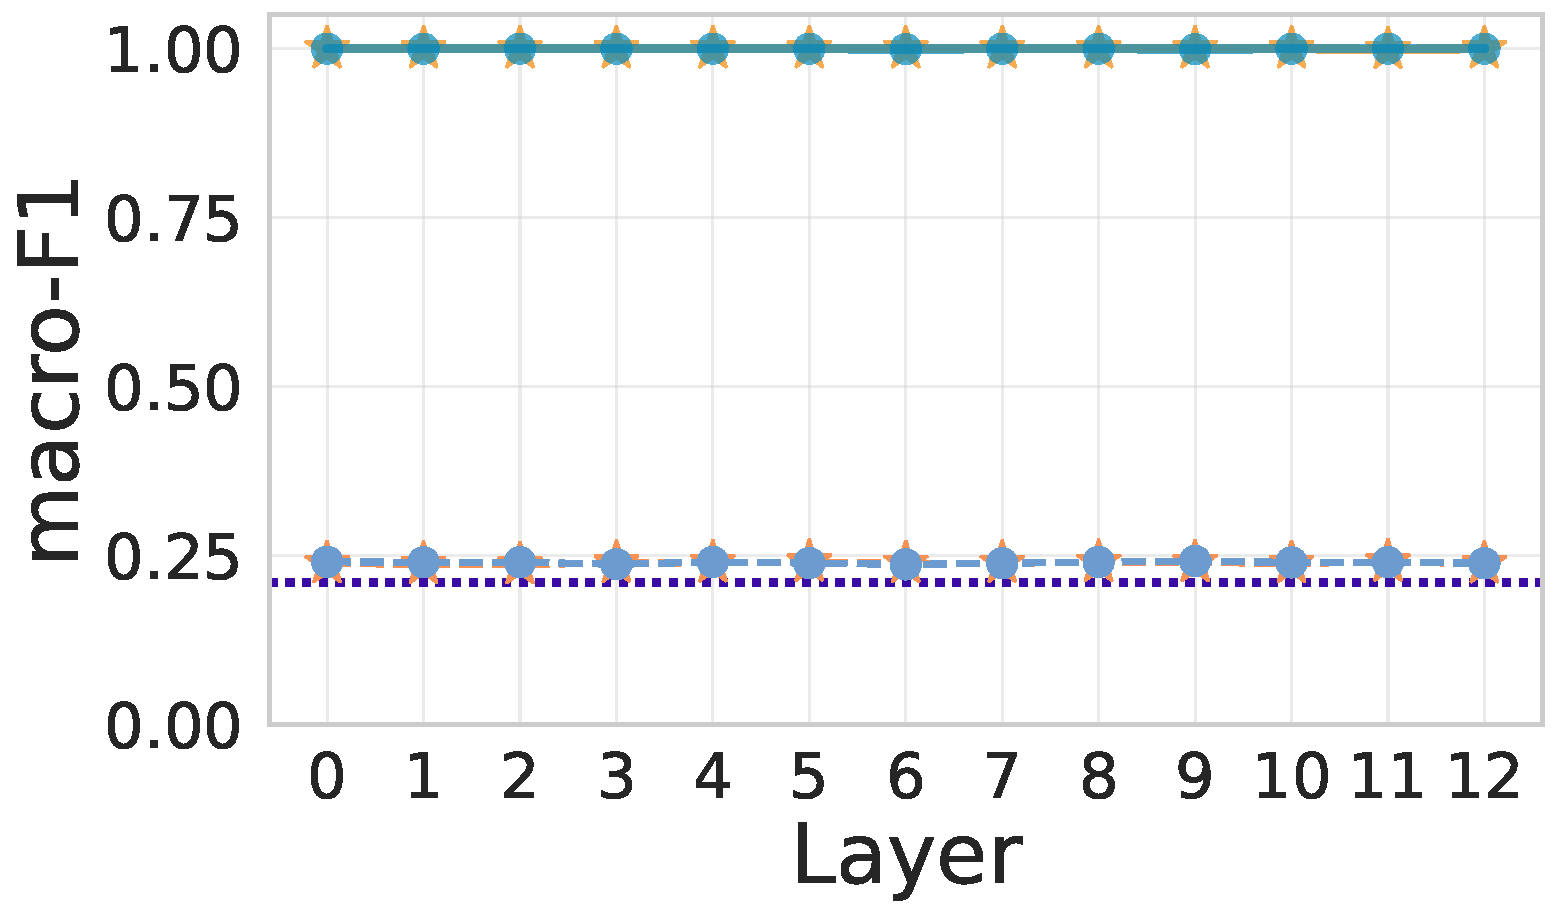
\includegraphics[width=\linewidth]{results_combined_f1/atom_type.pdf}
    \caption{atom type}
\end{subfigure}\hfill
\begin{subfigure}[t]{0.24\textwidth}
    \centering
    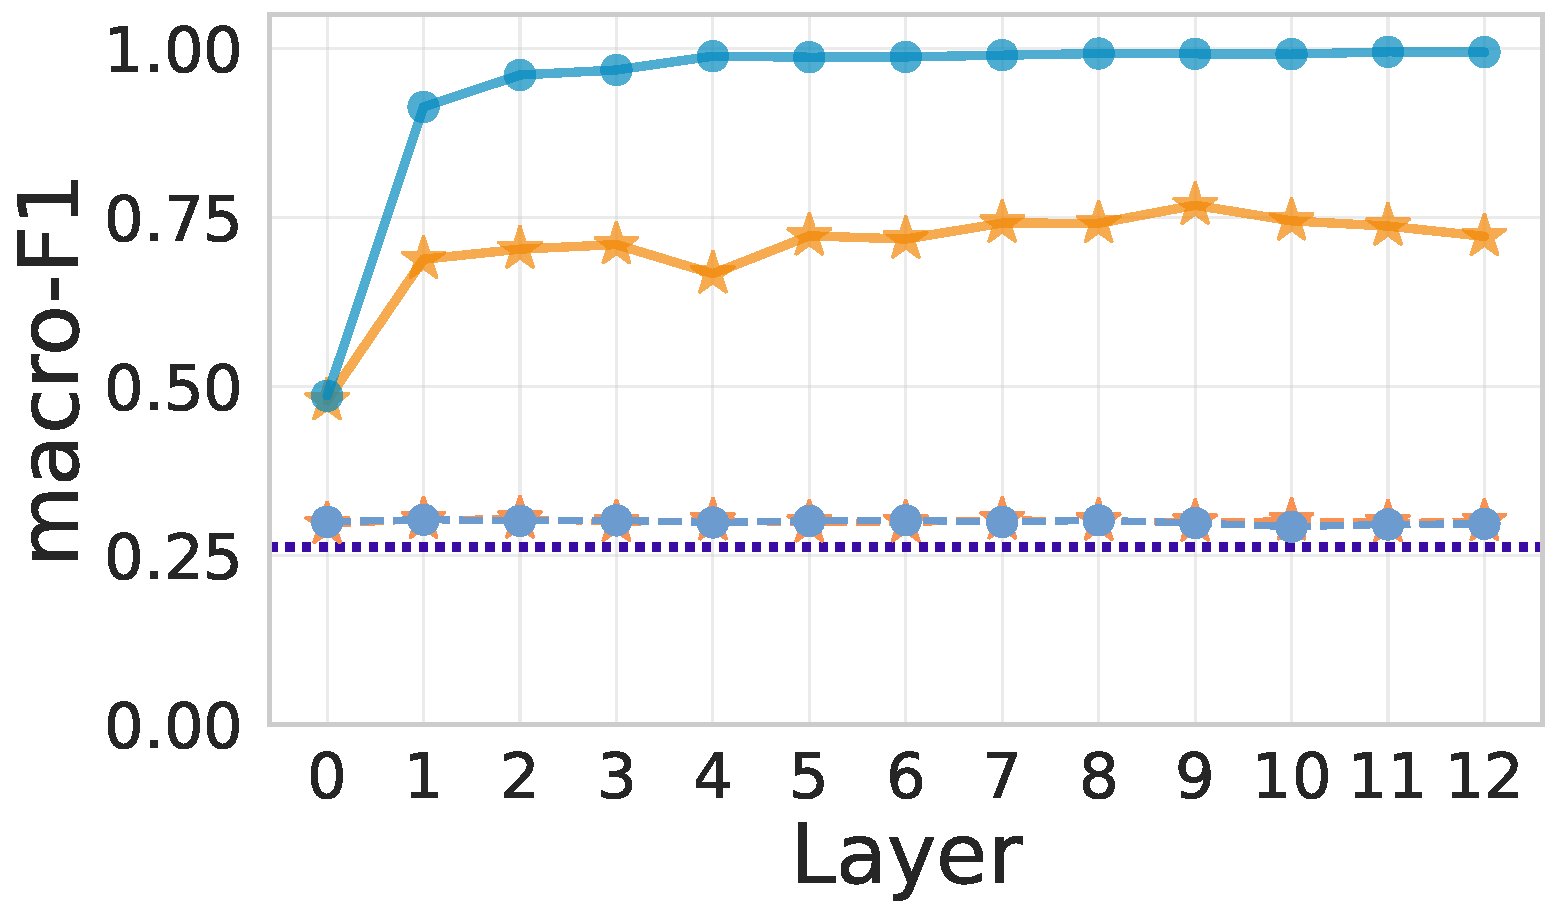
\includegraphics[width=\linewidth]{results_combined_f1/hybridization.pdf}
    \caption{hybridization}
\end{subfigure}\hfill
\begin{subfigure}[t]{0.24\textwidth}
    \centering
    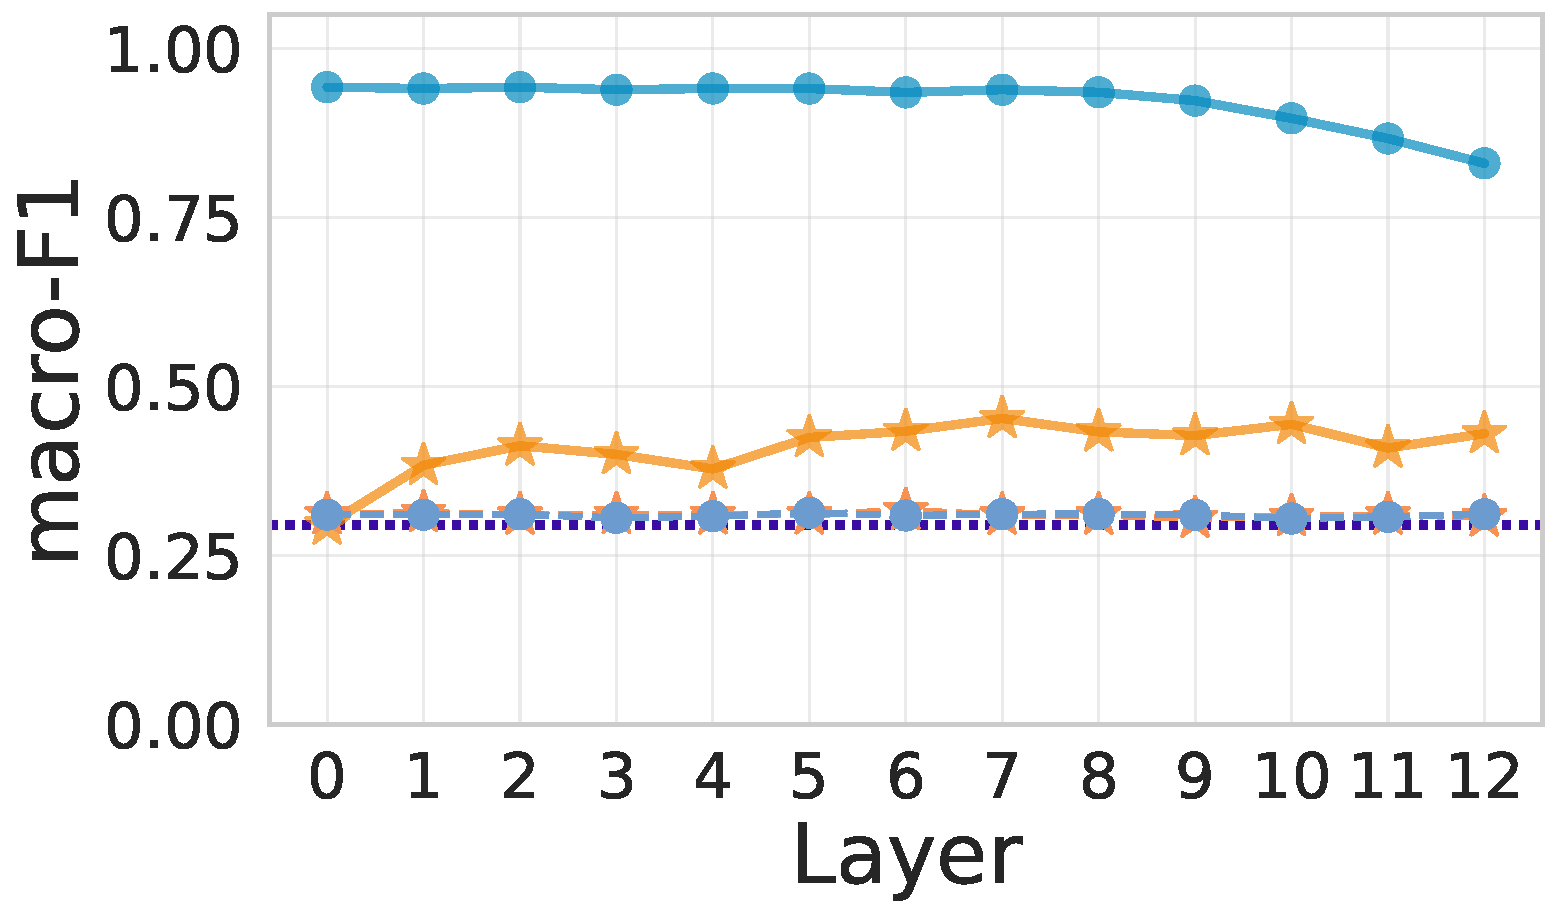
\includegraphics[width=\linewidth]{results_combined_f1/chiral_tag.pdf}
    \caption{chiral tag}
\end{subfigure}\hfill
\begin{subfigure}[t]{0.24\textwidth}
    \centering
    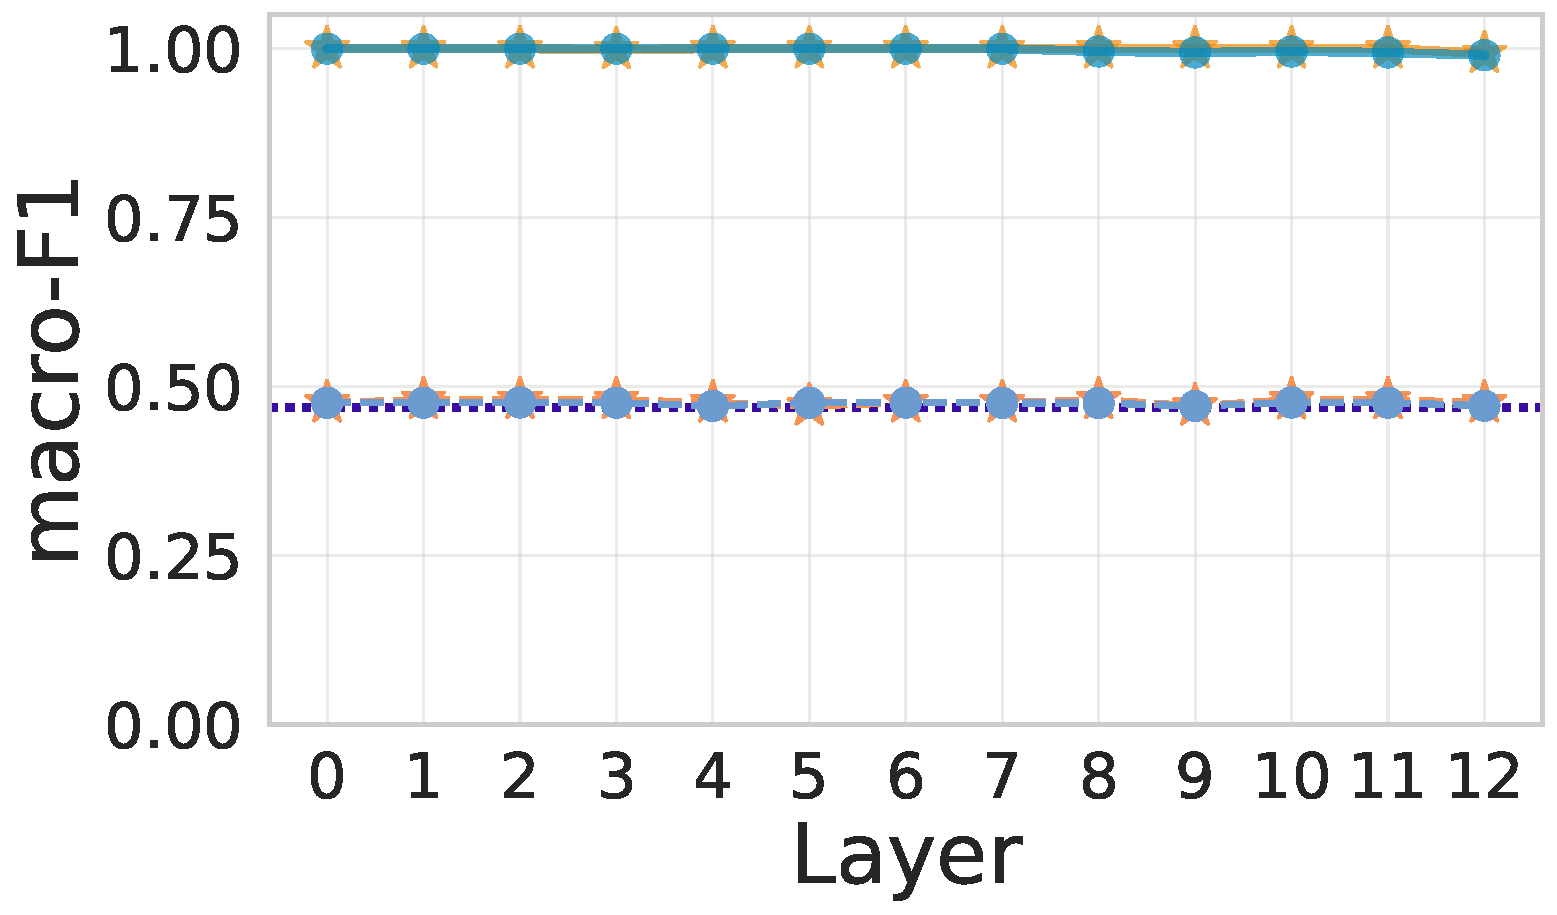
\includegraphics[width=\linewidth]{results_combined_f1/is_aromatic.pdf}
    \caption{is aromatic}
\end{subfigure}

\vspace{0.6em}

\begin{subfigure}[t]{0.24\textwidth}
    \centering
    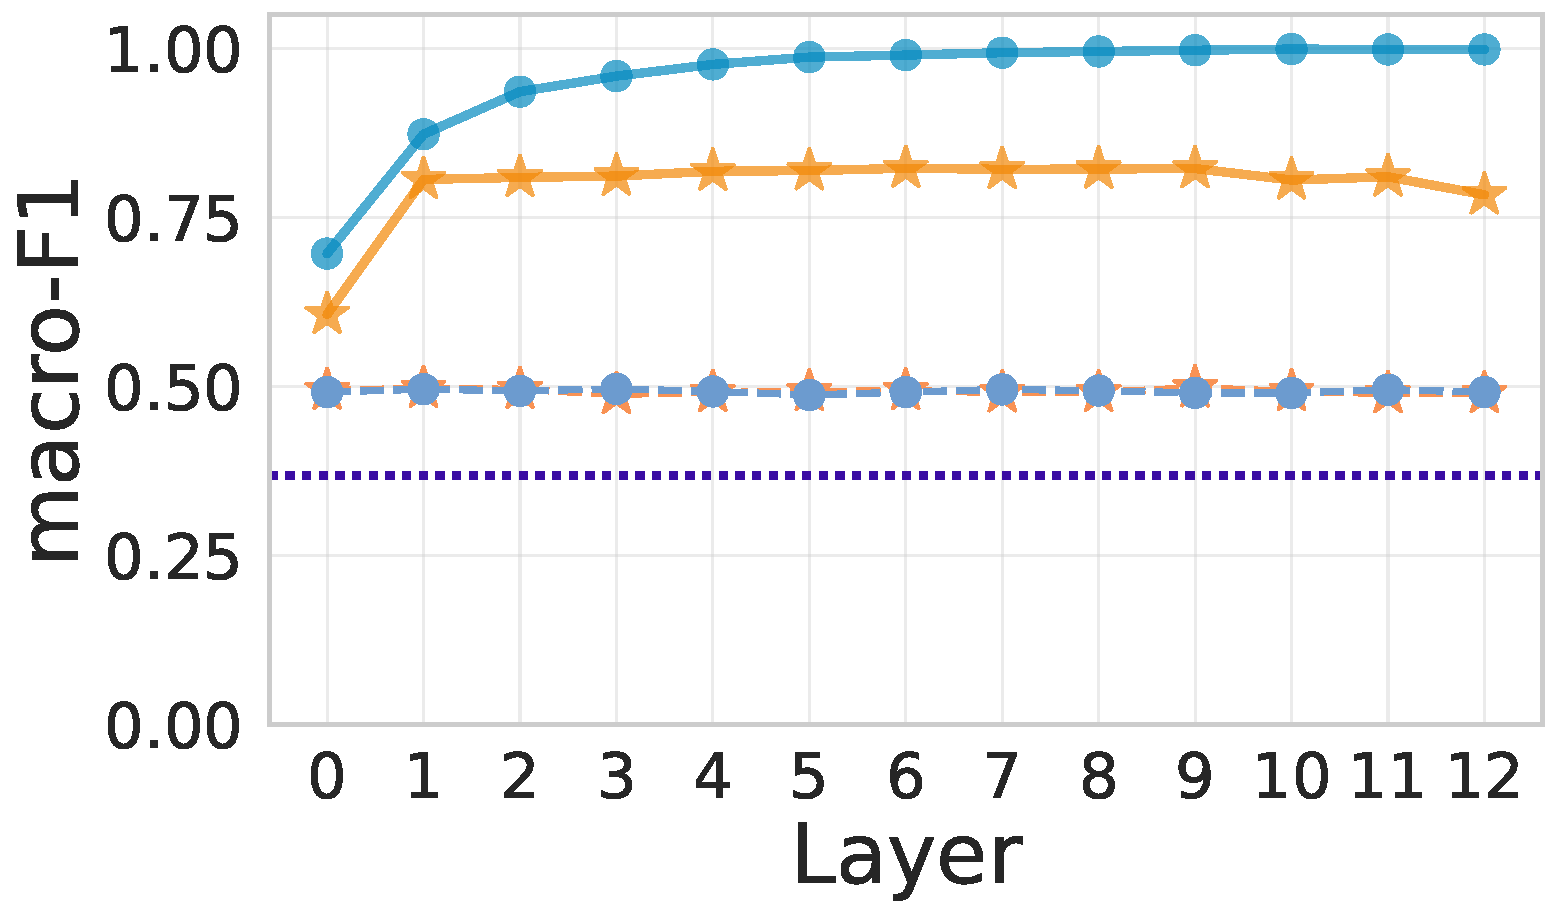
\includegraphics[width=\linewidth]{results_combined_f1/is_in_ring.pdf}
    \caption{is in ring}
\end{subfigure}\hfill
\begin{subfigure}[t]{0.24\textwidth}
    \centering
    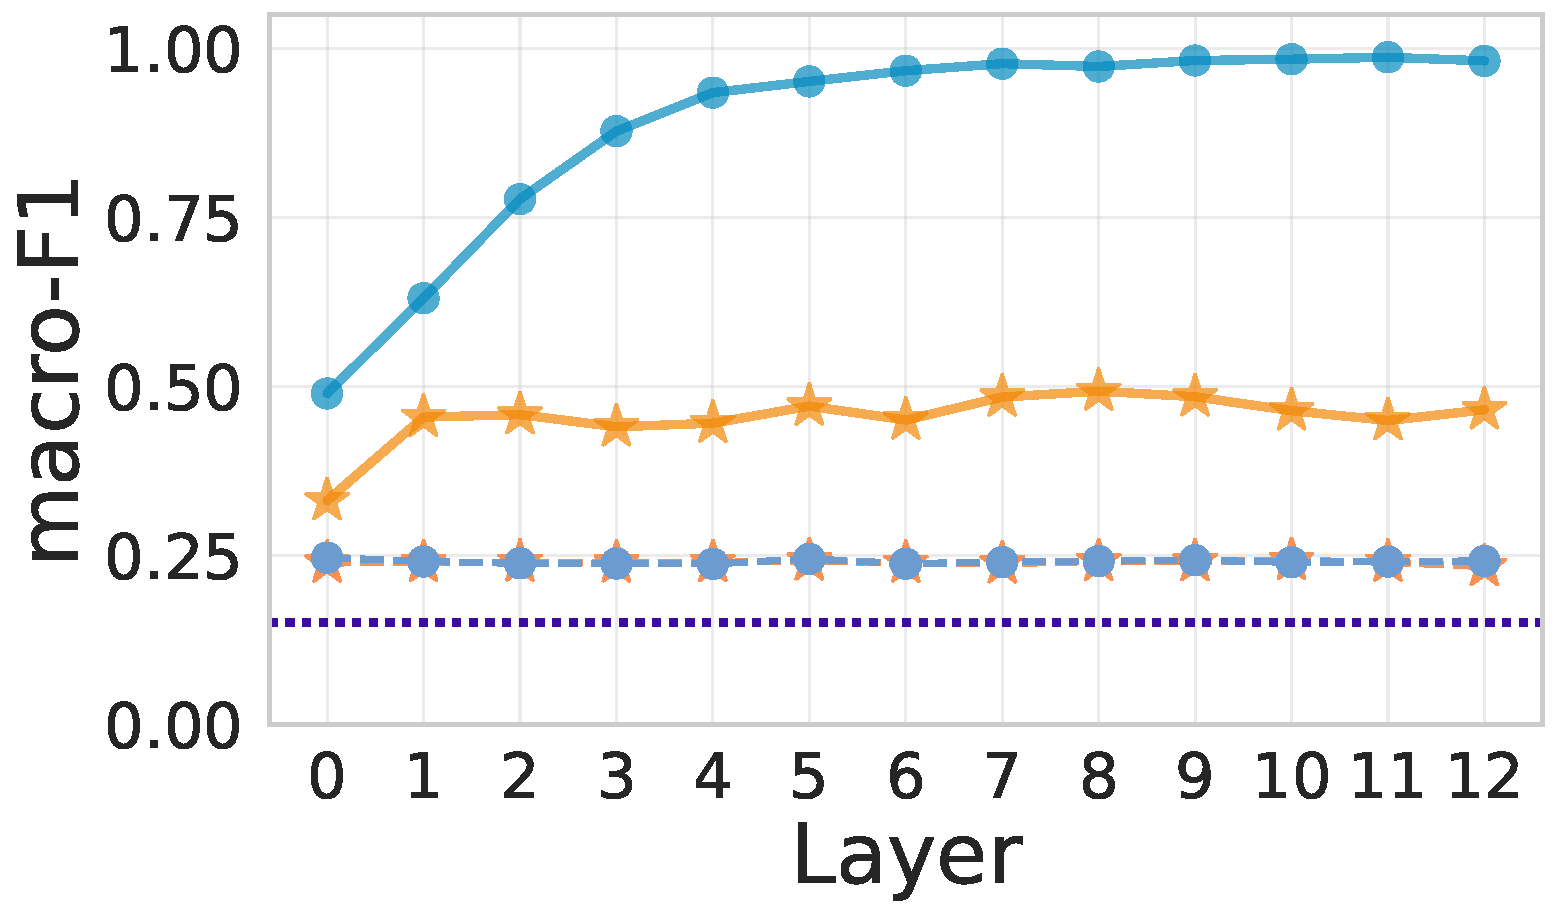
\includegraphics[width=\linewidth]{results_combined_f1/degree.pdf}
    \caption{degree}
\end{subfigure}\hfill
\begin{subfigure}[t]{0.24\textwidth}
    \centering
    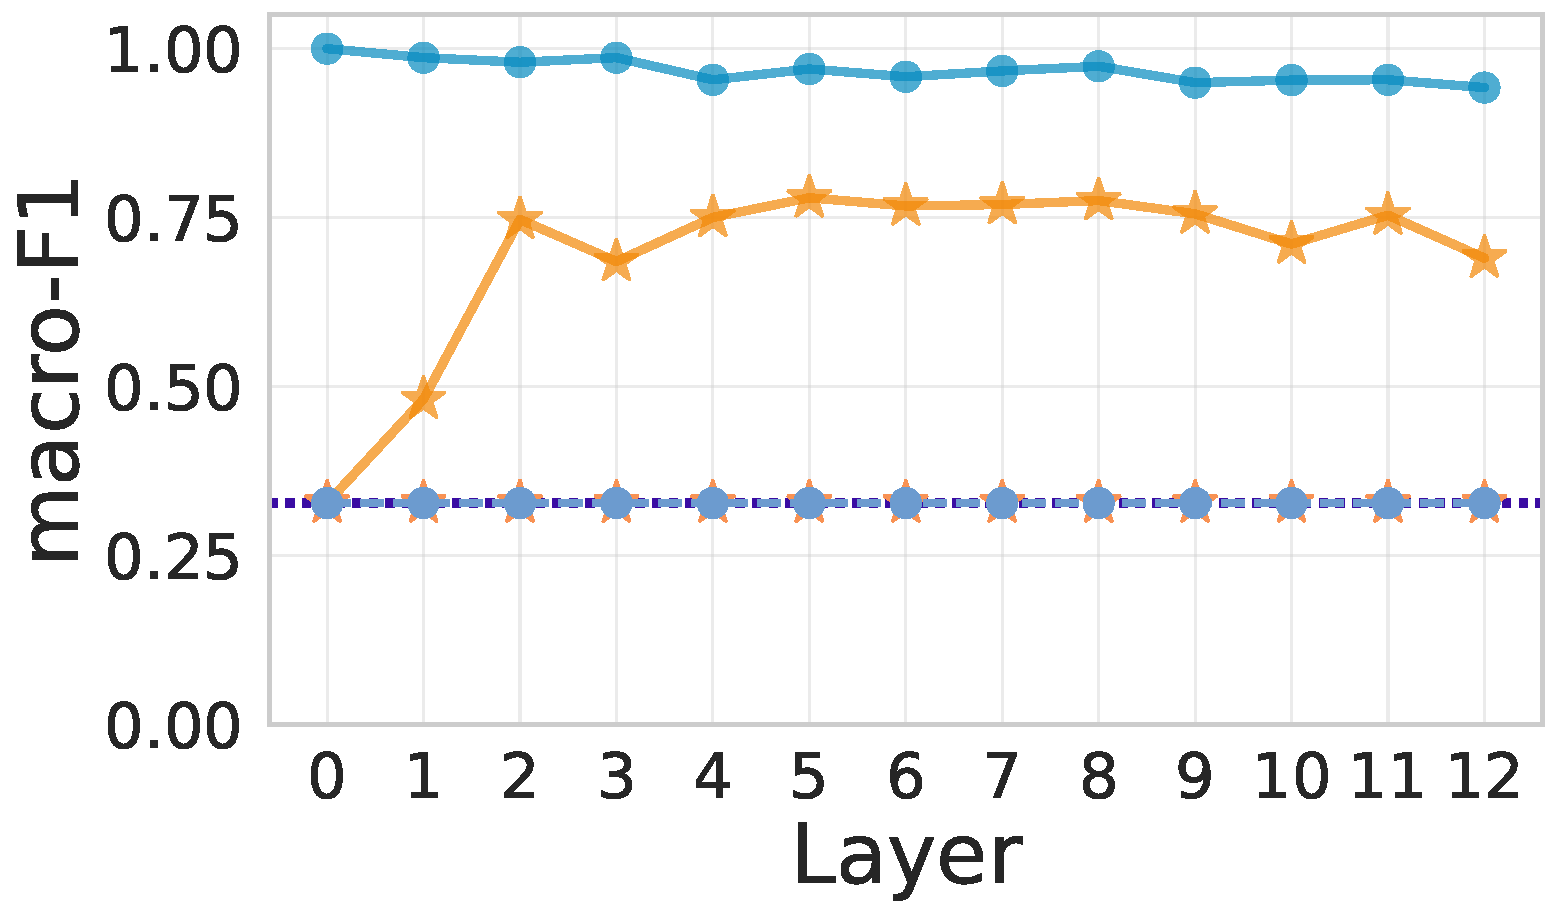
\includegraphics[width=\linewidth]{results_combined_f1/formal_charge.pdf}
    \caption{formal charge}
\end{subfigure}\hfill
\begin{subfigure}[t]{0.24\textwidth}
    \centering
    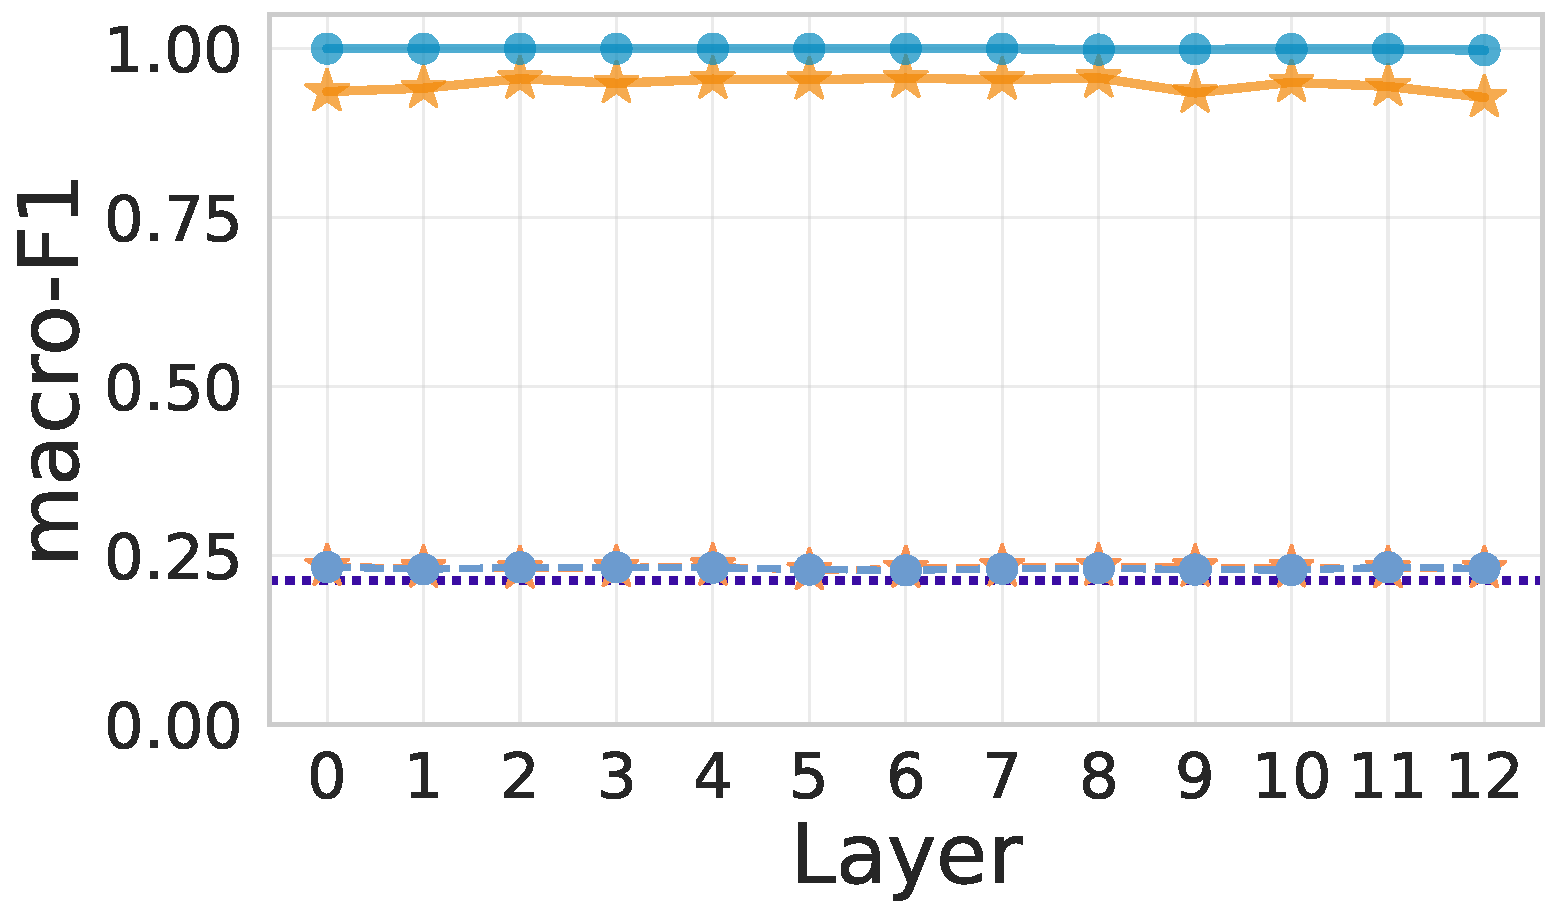
\includegraphics[width=\linewidth]{results_combined_f1/total_valence.pdf}
    \caption{total valence}
\end{subfigure}

\vspace{0.4em}

\centerline{
\includegraphics[width=0.95\textwidth]{results_combined_f1/legend.pdf}}

\caption{Per-layer linear-probe macro-F1 on the same eight tasks. Under macro-F1 \smi vs.\ \molm gap on contextual tasks is more pronounced than under accuracy, because macro-F1 penalises probes that effectively predict the majority class.}
\label{fig:f1}
\end{figure*}

\para{MLP-probe control.} To test whether the linear probe is bottlenecked by lack of nonlinearity, we additionally train a 2-layer MLP $\mathrm{MLPProbe}(\mathbf{x}) = \mathbf{W}_2\,\mathrm{ReLU}(\mathbf{W}_1\,\mathbf{x} + \mathbf{b}_1) + \mathbf{b}_2$ with hidden size $128$ on the real hidden states. Across all eight tasks and both models, the MLP probe improves test accuracy over the linear probe by at most $0.03$ in absolute terms, with most improvements being $\leq 0.01$. The largest gain is on \molm{} hybridization ($+0.03$ accuracy / $+0.07$ macro-F1 at layer $5$); on surface-form tasks the gap is essentially zero. We conclude that the chemical properties under study are approximately linearly accessible from the residual stream, and the conclusions drawn from the linear probe are not artifacts of probe capacity.

\para{Random-features control.} For each (task, layer) pair we additionally train an identical linear probe on a Gaussian random-features matrix $\mathbf{X}_{\mathrm{rand}} \in \mathbb{R}^{N \times d}$ with i.i.d.\ entries $\mathcal{N}(0, 1)$, sampled once per script run and reused for every (task, layer). The same molecule-level split, class encoding, and standardization are applied; the probe sees the same atom labels but uninformative inputs. Test macro-F1 falls within $1$--$2$ percentage points of $1/C_\tau$ (the chance level under macro-F1 when always predicting the majority class) for every task on both models, confirming that the real-features probe accuracy reflects encoder structure rather than overfitting capacity in the linear head.

\para{Macro-F1.} Figure~\ref{fig:f1} reports per-layer macro-F1 for six tasks for which it is informative (we omit atom type and formal charge, where the majority baseline is at or near $1.0$ and macro-F1 saturates). Under macro-F1 the \smi{} vs.\ \molm{} gap on contextual tasks is more pronounced than under accuracy, because macro-F1 penalizes probes that effectively reproduce the majority-vote baseline on imbalanced classes.

\subsection{Probe accuracy and steering for the remaining four properties}

The main text shows aromaticity, ring membership, degree, and chiral tag. Figure~\ref{fig:acc-all} and Figure~\ref{fig:steer-layer-all} report linear-probe accuracy and intervention success rate for the four remaining properties: atom type, hybridization, formal charge, and total valence. Atom type and formal charge are surface-form (or near-surface-form, since the majority baseline of formal charge is already $0.97$): both models reach the same near-saturation accuracy at the embedding and layer-sweep success curves are dominated by probe-prototype geometry on the multi-class cycle target. Hybridization and total valence are contextual; \smi{} reaches near-perfect probe accuracy and intervention success by mid-layers, while \molm{} plateaus several points below on probing and lifts only at the deepest layers under intervention---the same shape we see for the contextual tasks in the main text.

\begin{figure}[t]
\centering
\begin{subfigure}[t]{0.24\linewidth}
    \centering
    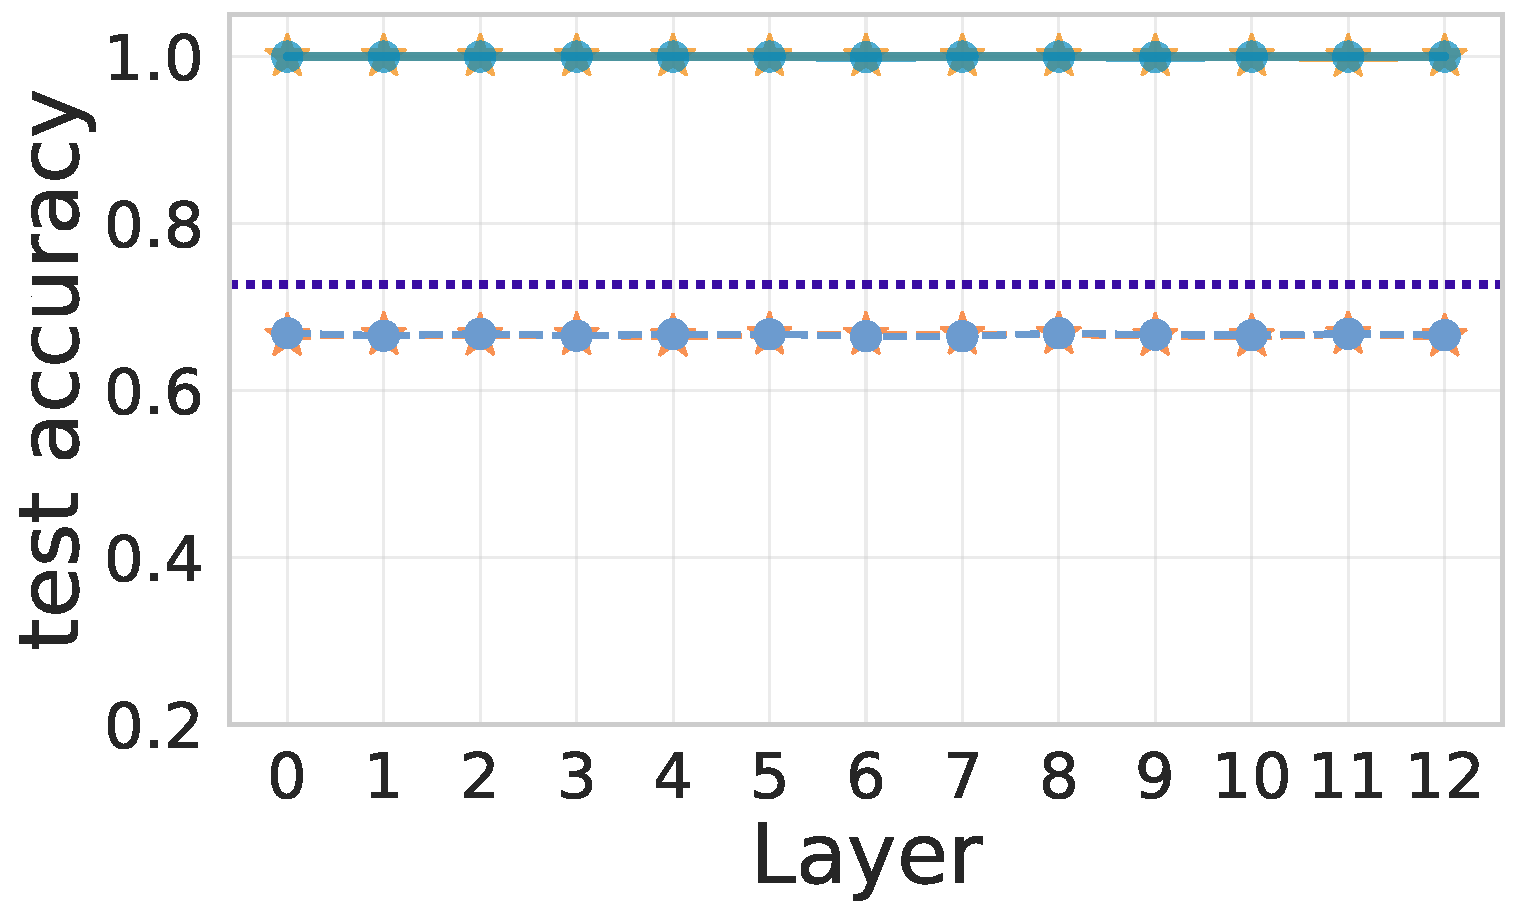
\includegraphics[width=\linewidth]{results_combined/atom_type.pdf}
    \subcaption{atom type}
    \label{fig:acc-all-atom-type}
\end{subfigure}\hfill
\begin{subfigure}[t]{0.24\linewidth}
    \centering
    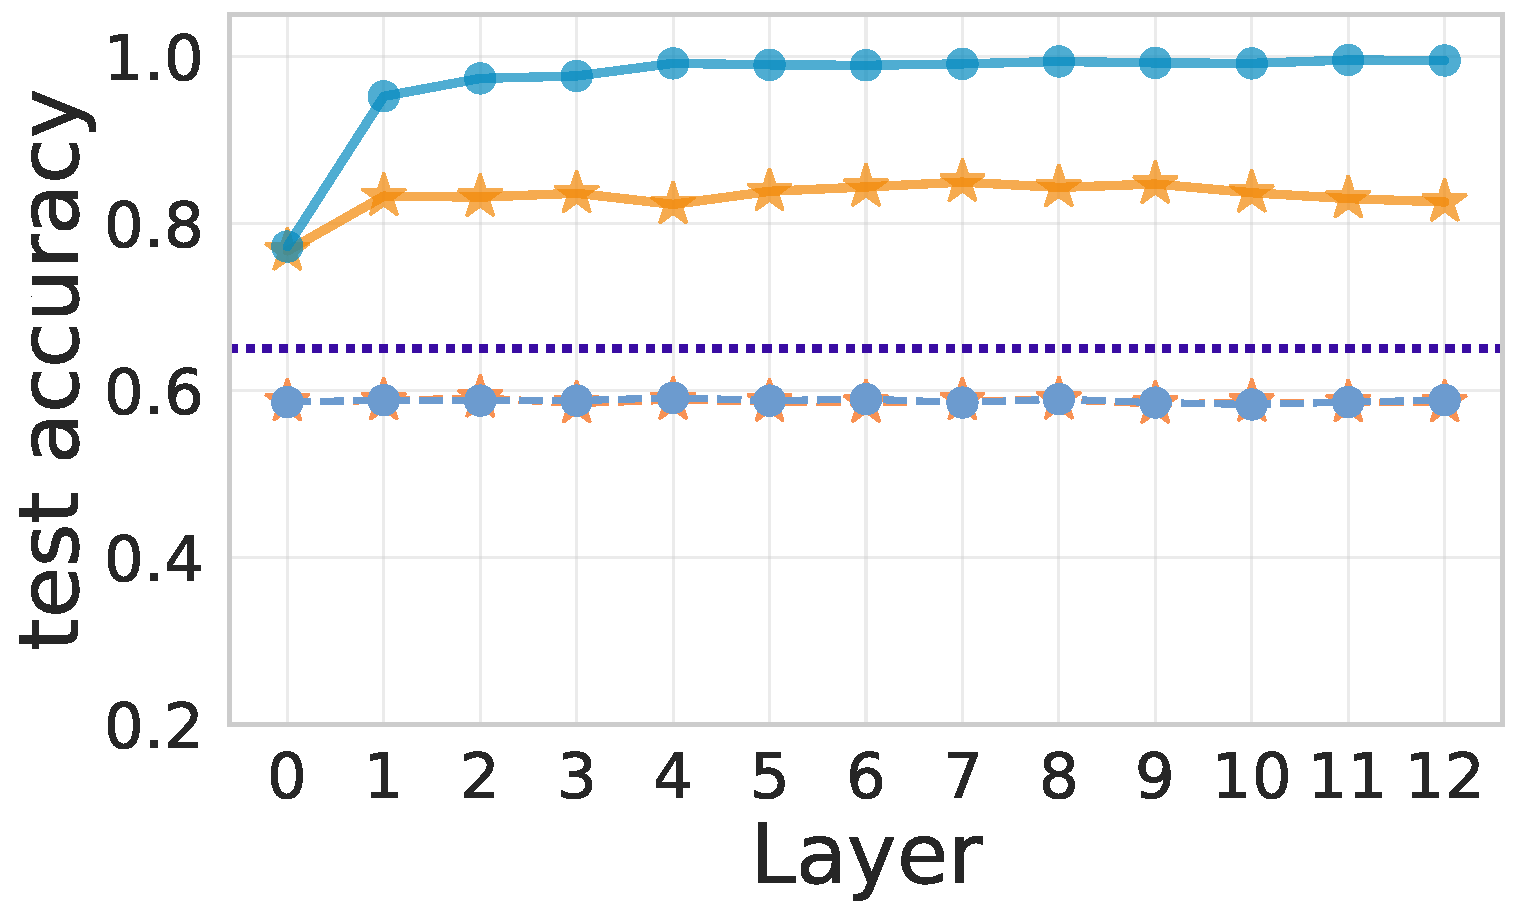
\includegraphics[width=\linewidth]{results_combined/hybridization.pdf}
    \subcaption{hybridization}
    \label{fig:acc-all-hybridization}
\end{subfigure}\hfill
\begin{subfigure}[t]{0.24\linewidth}
    \centering
    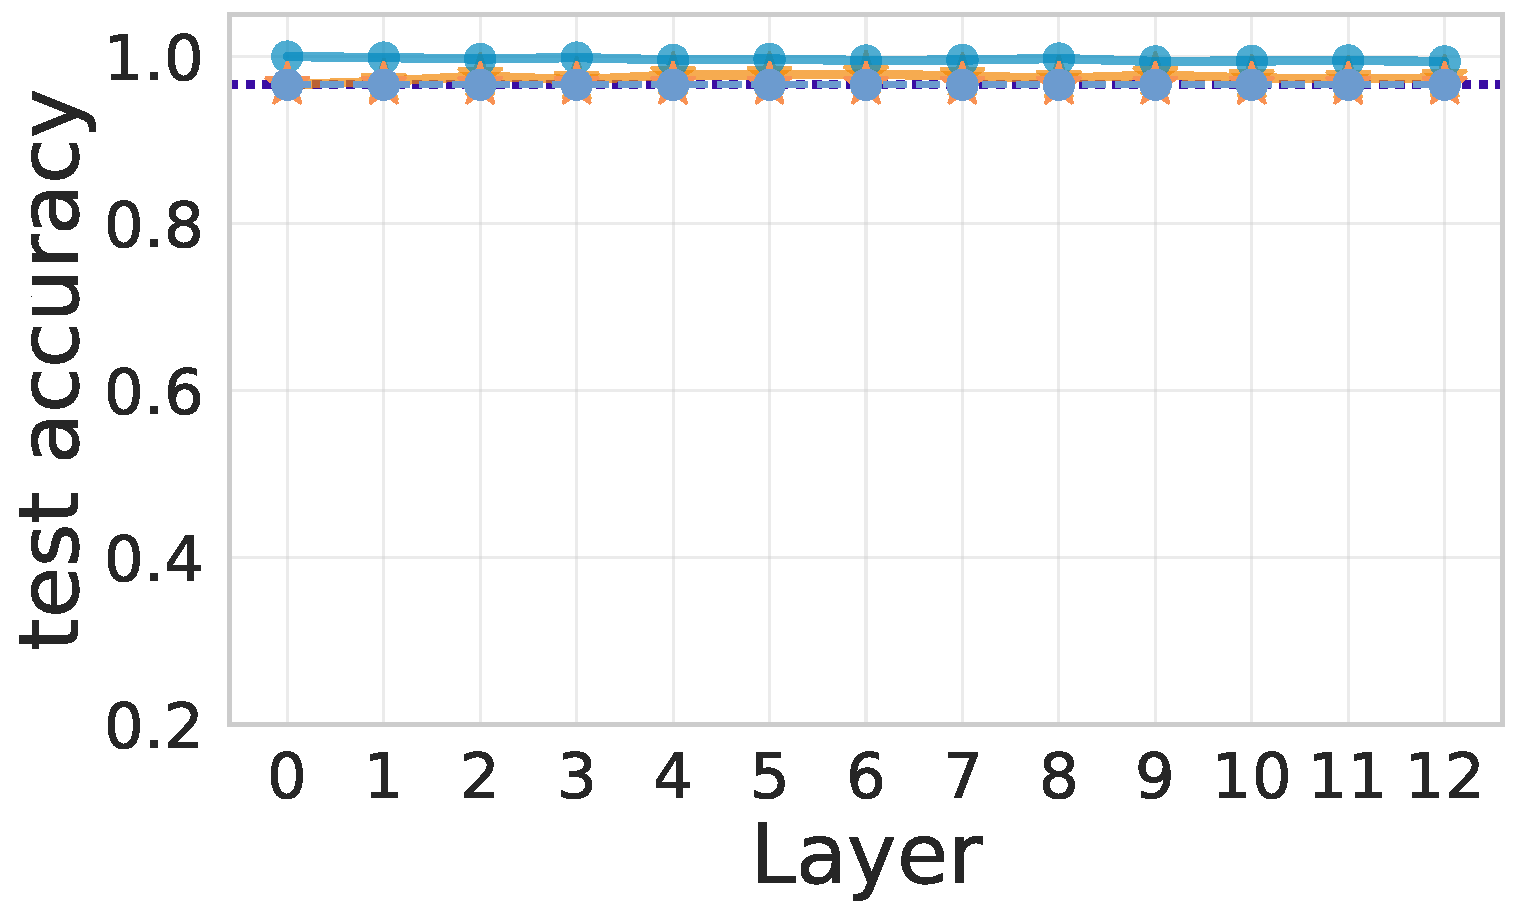
\includegraphics[width=\linewidth]{results_combined/formal_charge.pdf}
    \subcaption{formal charge}
    \label{fig:acc-all-formal-charge}
\end{subfigure}\hfill
\begin{subfigure}[t]{0.24\linewidth}
    \centering
    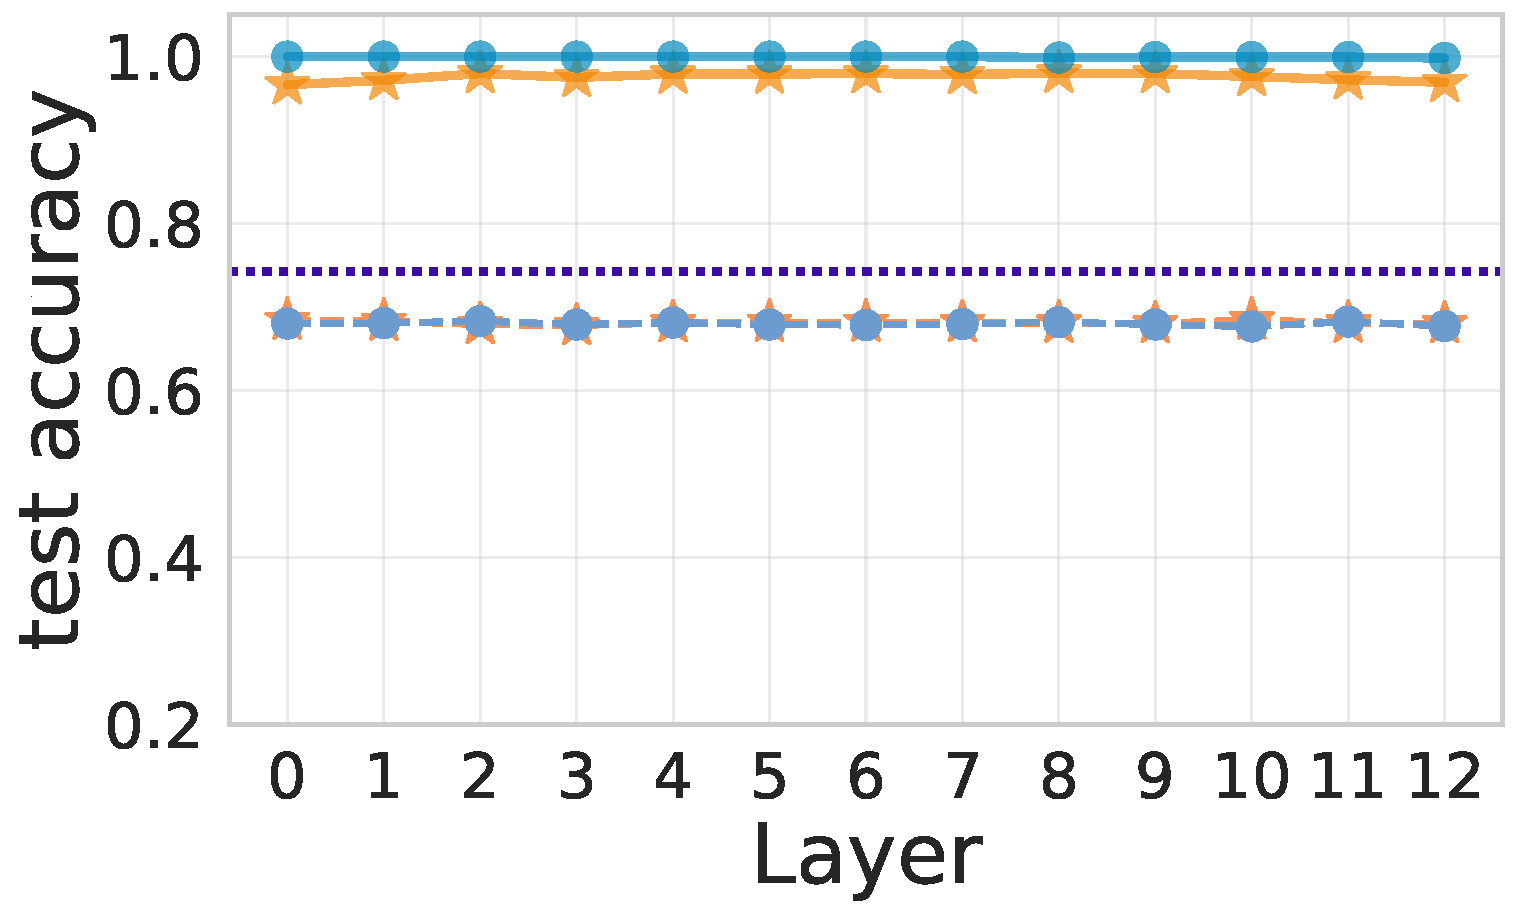
\includegraphics[width=\linewidth]{results_combined/total_valence.pdf}
    \subcaption{total valence}
    \label{fig:acc-all-total-valence}
\end{subfigure}

\vspace{0.4em}

\centerline{
\includegraphics[width=0.85\linewidth]{results_combined/legend.pdf}}

\caption{Linear-probe test accuracy per layer for the four properties not shown in the main text. Atom type (\ref{fig:acc-all-atom-type}) is surface-form and saturates at $1.0$ from layer~$0$ in both models. Formal charge (\ref{fig:acc-all-formal-charge}) is similarly close to its $0.97$ majority baseline in both models from the embedding onward. Hybridization (\ref{fig:acc-all-hybridization}) and total valence (\ref{fig:acc-all-total-valence}) are contextual and follow the same pretraining-difference shape as ring membership, degree, and chiral tag in the main text: \smi reaches near-perfect accuracy by mid-layers while \molm plateaus several points below.}
\label{fig:acc-all}
\end{figure}
\begin{figure}[t]
\centering
\begin{subfigure}[t]{0.48\linewidth}
    \centering
    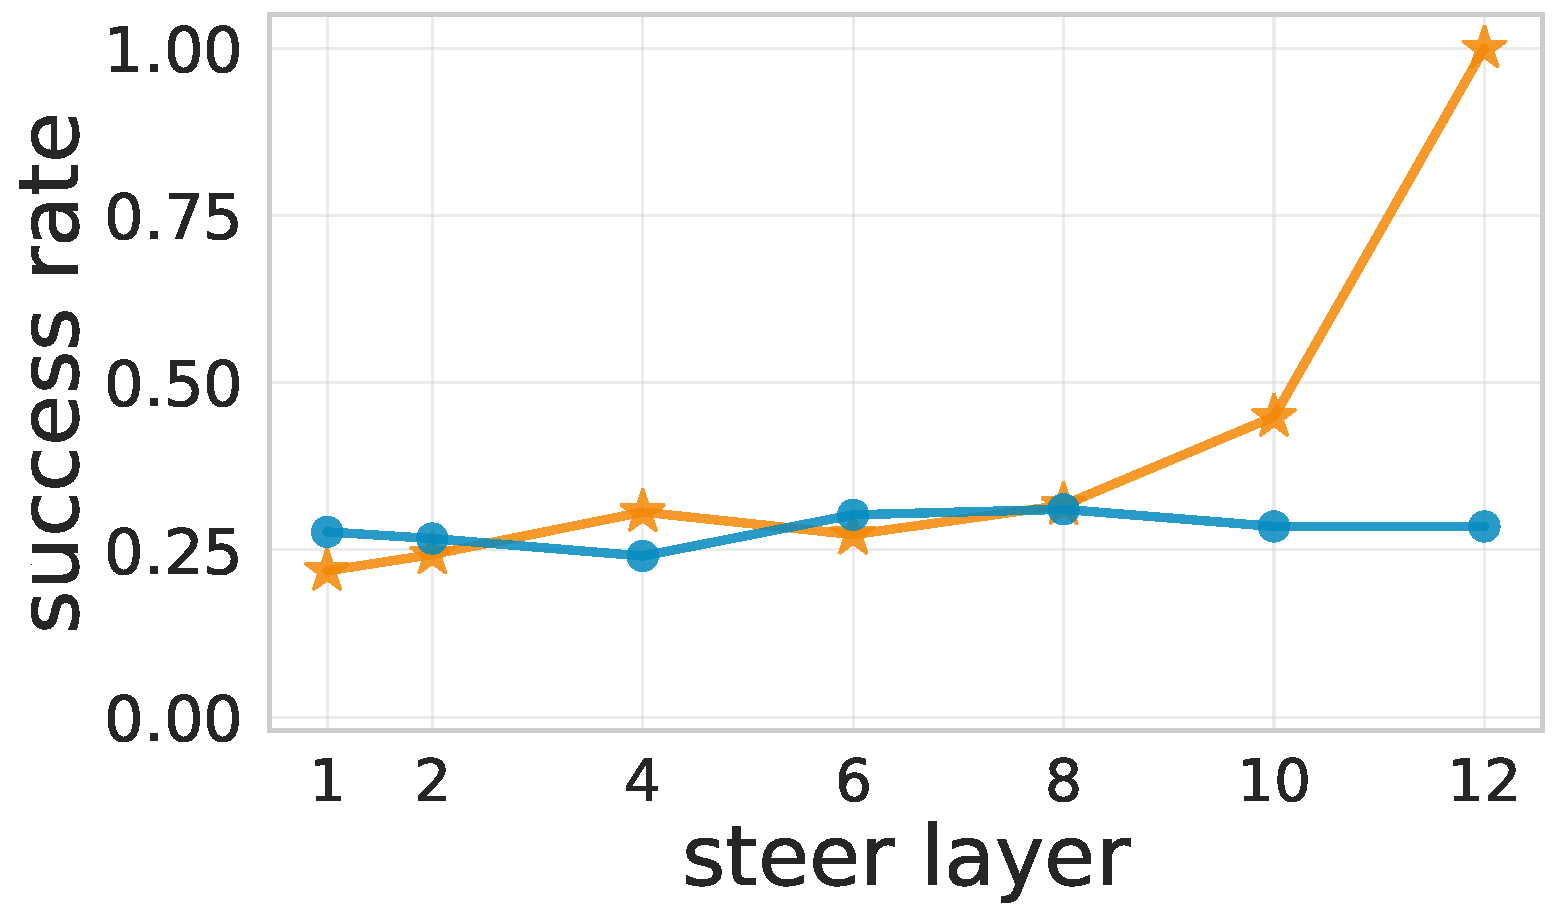
\includegraphics[width=\linewidth]{results_steer_layers/by_layer_atom_type.pdf}
    \subcaption{atom type}
    \label{fig:steer-all-atom-type}
\end{subfigure}\hfill
\begin{subfigure}[t]{0.48\linewidth}
    \centering
    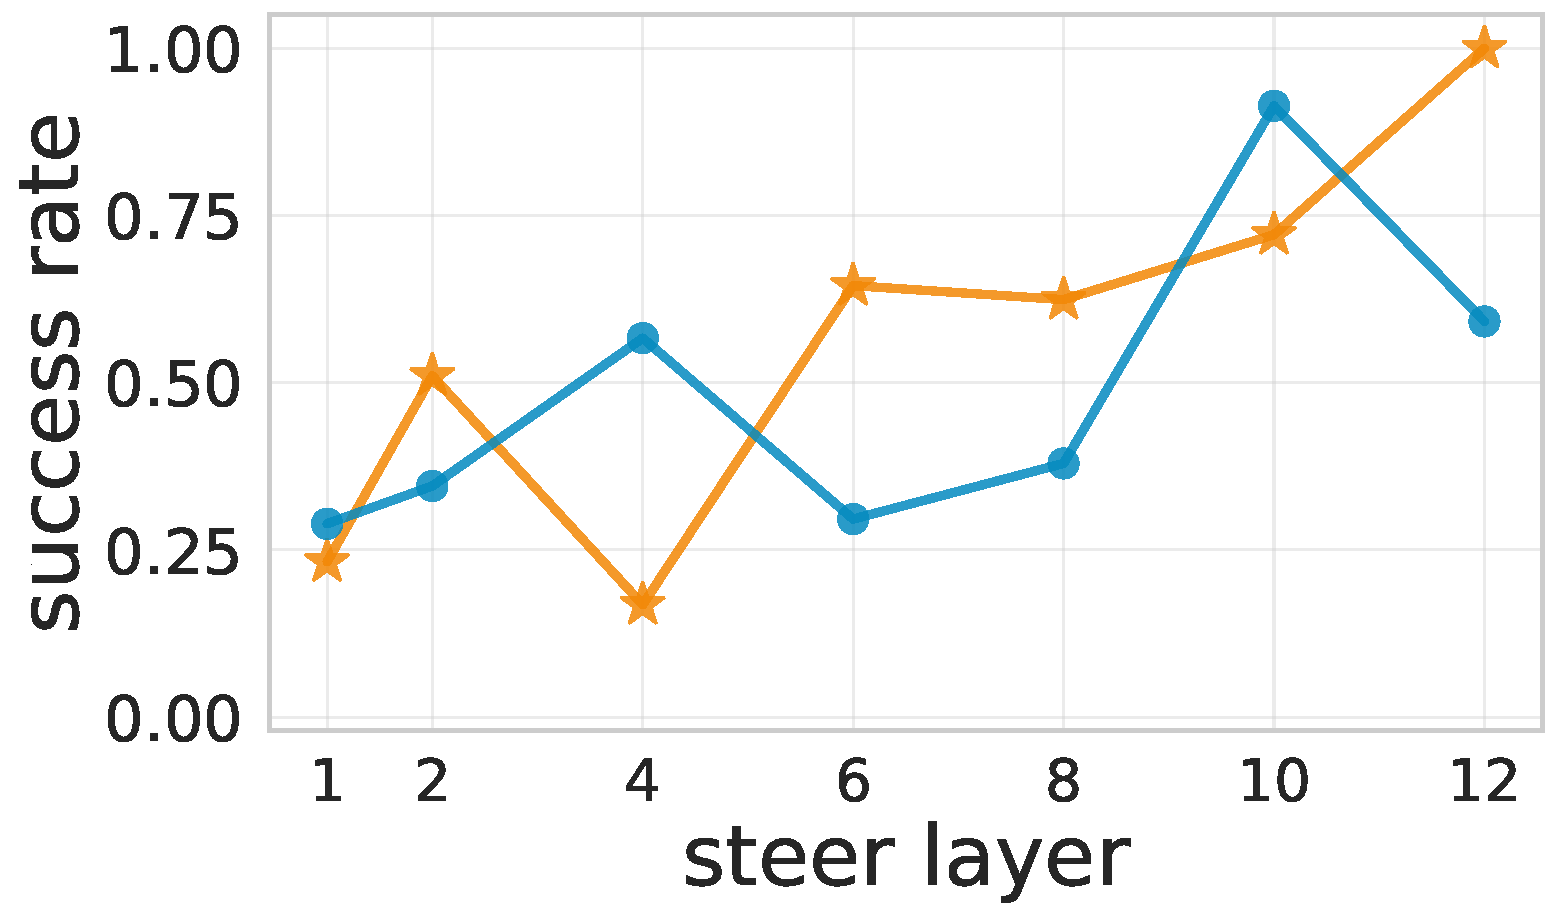
\includegraphics[width=\linewidth]{results_steer_layers/by_layer_hybridization.pdf}
    \subcaption{hybridization}
    \label{fig:steer-all-hybridization}
\end{subfigure}

\vspace{0.6em}

\begin{subfigure}[t]{0.48\linewidth}
    \centering
    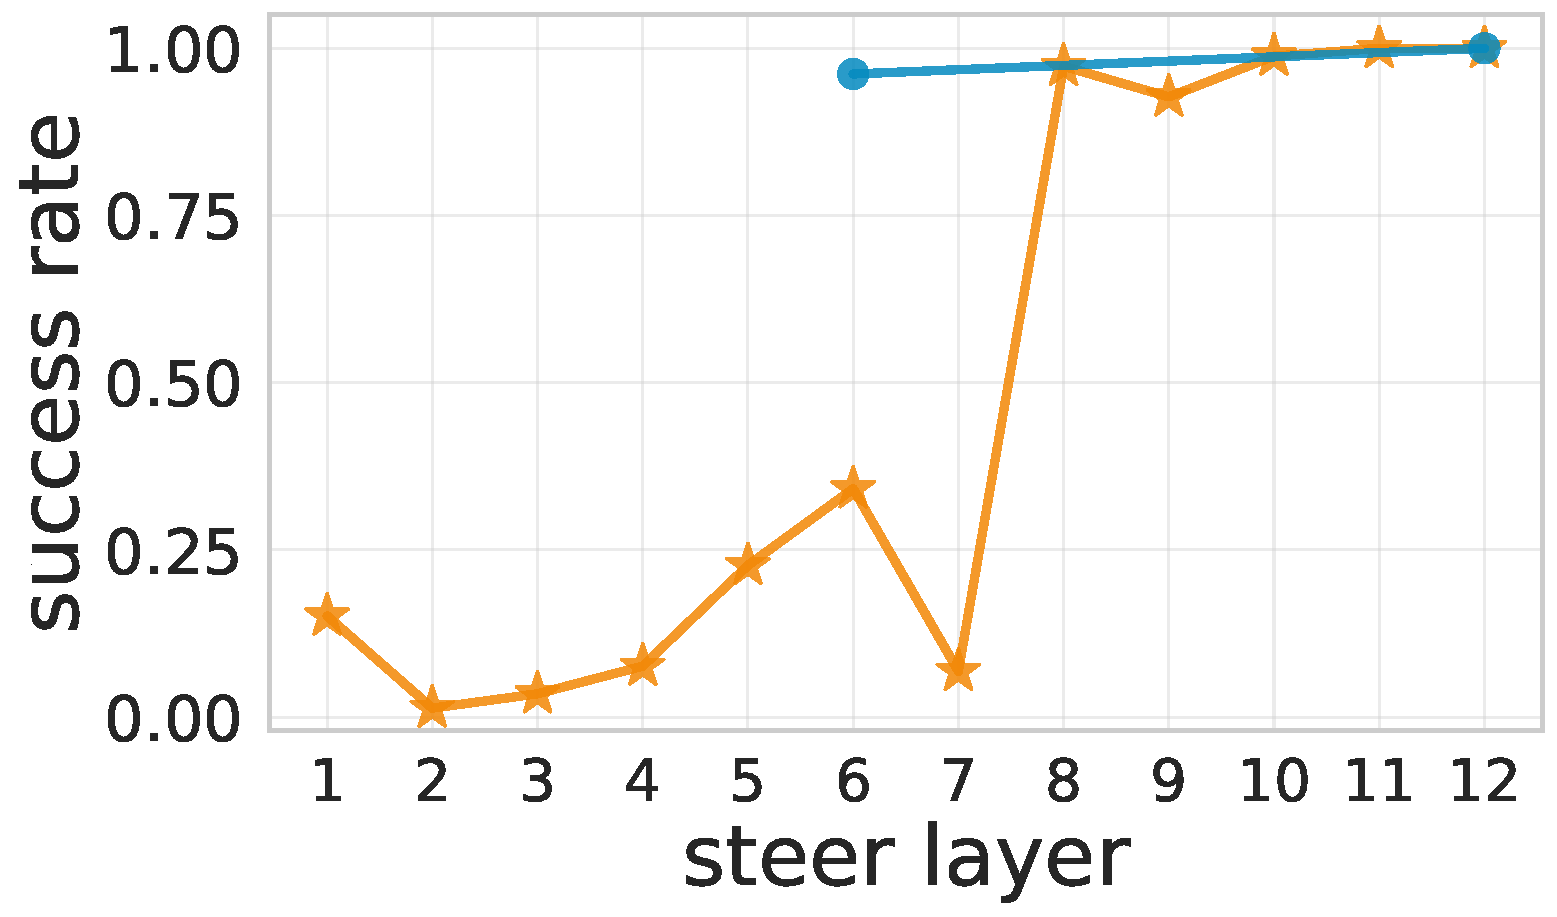
\includegraphics[width=\linewidth]{results_steer_layers/by_layer_formal_charge.pdf}
    \subcaption{formal charge}
    \label{fig:steer-all-formal-charge}
\end{subfigure}\hfill
\begin{subfigure}[t]{0.48\linewidth}
    \centering
    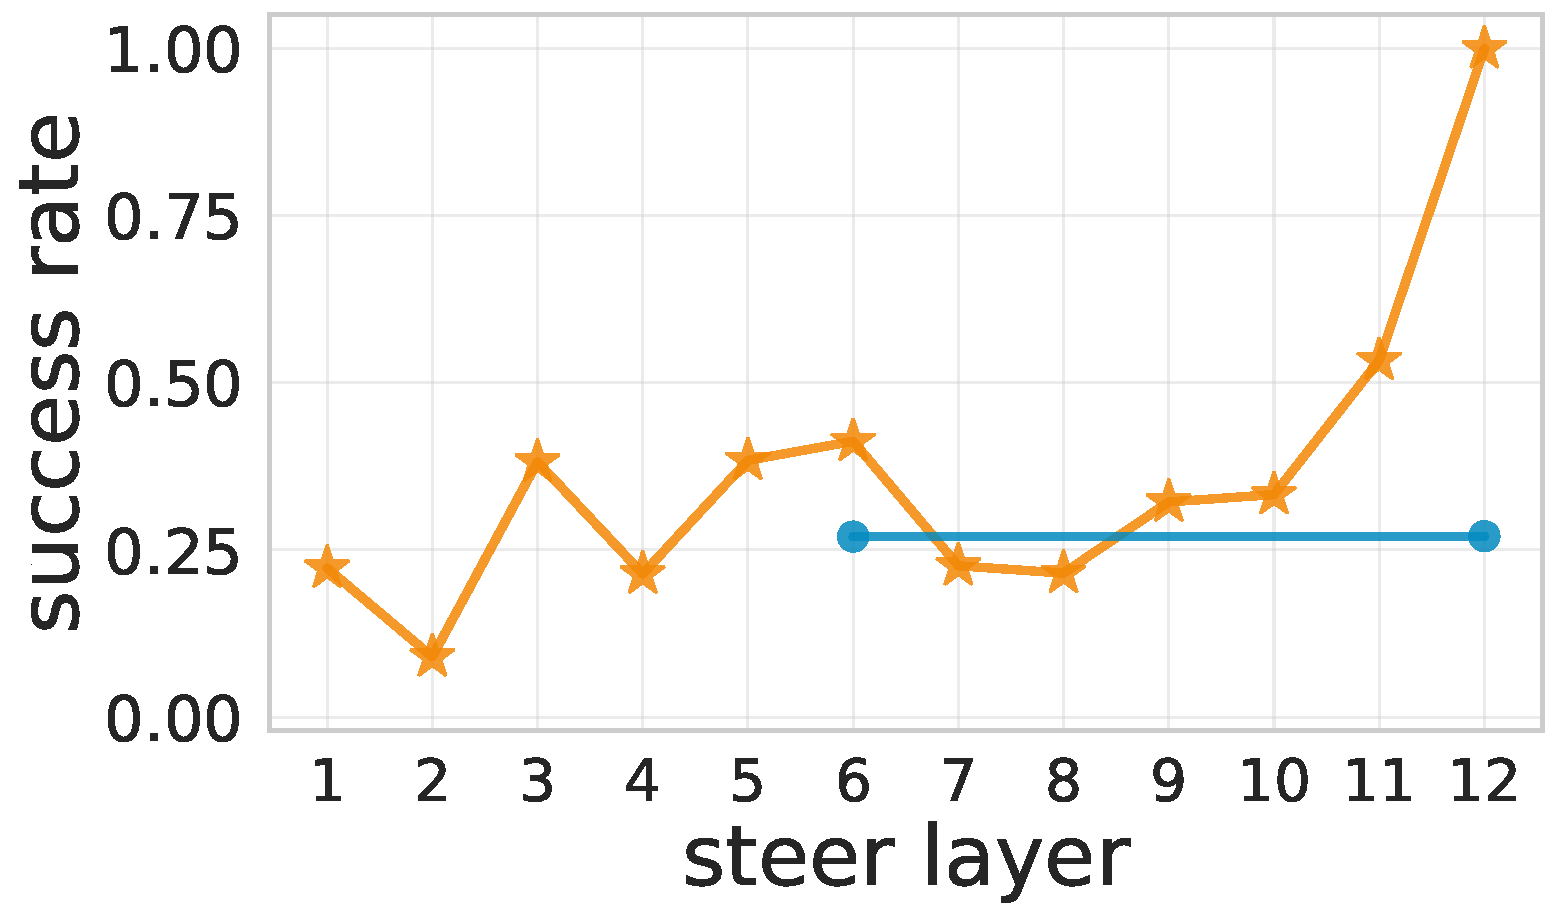
\includegraphics[width=\linewidth]{results_steer_layers/by_layer_total_valence.pdf}
    \subcaption{total valence}
    \label{fig:steer-all-total-valence}
\end{subfigure}

\vspace{0.4em}

\centerline{
\includegraphics[width=0.5\linewidth]{results_steer_layers/by_layer_legend.pdf}}

\caption{Intervention success rate as a function of the steer layer for the four properties not shown in the main text. Formal charge (\ref{fig:steer-all-formal-charge}) follows the same pretraining-difference shape seen in the main text: \smi saturates at high success by mid-layers, \molm climbs gradually until the top of the encoder. Atom type (\ref{fig:steer-all-atom-type}), hybridization (\ref{fig:steer-all-hybridization}), and total valence (\ref{fig:steer-all-total-valence}) are multi-class targets and the cycle-target success rate is partly governed by the probe-prototype layout; we therefore additionally inspect the moved-off-source rate (Appendix~\ref{app:steering}) to disentangle ``the intervention had effect'' from ``the intervention hit the cycle target''.}
\label{fig:steer-layer-all}
\end{figure}


\subsection{Causal-steering setup}

\para{Steering vector.} For each (task, steer layer $\ell$) we form, in the original (unstandardized) hidden-state space,
\[
\mathbf{v}^{c \to c'} = (\mathbf{W}_{c'} - \mathbf{W}_{c}) / \boldsymbol{\sigma},
\]
where $\mathbf{W}_{c}$ is the layer-$\ell$ probe's row for class $c$ and $\boldsymbol{\sigma}$ is the per-feature training standard deviation. Adding $\alpha \cdot \mathbf{v}^{c \to c'}$ to a hidden state increases the standardized logit difference $\mathrm{logit}_{c'} - \mathrm{logit}_{c}$ by $\alpha \cdot \|\mathbf{W}_{c'} - \mathbf{W}_c\|_{\boldsymbol{\sigma}^{-2}}^2$. For binary tasks, $\mathrm{tgt} = 1 - \mathrm{src}$. For multi-class tasks, we use a cycle target $\mathrm{tgt} = (\mathrm{src} + 1) \bmod C_\tau$.

\para{Forward hook and intervention.} The hook is registered on the module that produces $\mathbf{h}^{(\ell)}$ (\texttt{model.encoder.layer[$\ell$-1]} for \molm{}, \texttt{encoder.blocks.layers[$\ell$-1]} for \smi{}), modifies that layer's output by adding the per-position steering tensor at atom-token positions only, and is removed in a \texttt{try/finally} block immediately after the post-intervention forward pass. The pre- and post-intervention forward passes are run with \texttt{output\_hidden\_states=True} to capture the residual stream at every depth.

\para{Layer sweep.} The main-text Figure~\ref{fig:steer-layer} and the appendix Figure~\ref{fig:steer-layer-all} sweep $\ell \in \{1, \ldots, 12\}$ and report, per (task, model, $\ell$), the intervention success rate at the best-performing $\alpha$ on held-out molecules. This best-$\alpha$-per-layer summary serves as a single scalar diagnostic of whether the encoder routes through the layer-$\ell$ probe direction.

\para{Metrics.} \emph{Intervention success rate} (or \emph{flip-to-target rate}) is the fraction of atom-token positions whose layer-$12$ probe prediction equals the intended target $c'$ after the intervention. We additionally track \emph{moved-off-source rate} (the fraction whose post-intervention layer-$12$ prediction differs from the source class $c$) so that, for multi-class tasks, ``the steering had effect'' can be disentangled from ``the steering hit the cycle target''---a distinction that matters when the cycle direction $\mathbf{W}_{c'} - \mathbf{W}_{c}$ does not point at the cycle-target centroid in the probe's prototype layout.

\para{Sample size and hyperparameters.} Each task is evaluated on $200$ molecules ($\sim 1.7$k atom-token positions; $197$ molecules and $1{,}719$ atom-token positions survive token-atom alignment) drawn from the QM9 partition not used for probe training. The $\alpha$ grid is $\{0, 1, 3, 10, 30, 100, 300\}$; the smallest non-zero $\alpha$ that maximizes success rate is reported per layer.


\end{document}
